\documentclass{article}
\usepackage[T2A]{fontenc}
\usepackage{fontspec}
\setmainfont{CMU Serif}
\usepackage[russian]{babel}
\usepackage{graphicx}
\usepackage{cancel}
\usepackage{bm}
%math packages
\usepackage{amsmath}
\usepackage{amsthm}
\usepackage{amssymb}
\usepackage{latexsym}
\usepackage{geometry}
\geometry{a4paper,scale=0.8}
\usepackage[pdfborder=000]{hyperref}
%define numbers with circles
\usepackage{tikz}
\newcommand*{\circled}[1]{\lower.7ex\hbox{\tikz\draw (0pt, 0pt)%
		circle (.5em) node {\makebox[1em][c]{\small #1}};}}

\newtheorem{example}{Пример}
\newtheorem{question}{Вопрос}
\newtheorem{Remark}{Замечание}
\newtheorem{theorem}{Теорема}
\newtheorem{definition}{Определение}
\newtheorem{proposition}{Утверждение}
\numberwithin{example}{section}
\numberwithin{question}{section}
\numberwithin{Remark}{section}
\numberwithin{theorem}{section}
\numberwithin{definition}{section}
\numberwithin{proposition}{section}
\begin{document}
\section{Лекция 1}
$X=\{x_1,x_2,\ldots,x_n,\ldots \}$ - \textbf{алфавит}. Символы $x_i\in X$ называем \textbf{буквами} (над алфавитом $X$).\\
Любая конечная последовательность бкув $x_1,x_2,\ldots,x_n$ называется \textbf{словом} (над алфавитом $X$). \\
Число символов из $X$ в слове называются \textbf{длиной слова}. Само слово может обозначается символом $\tilde{x}$, а длина слова обозначается символом $l$.
\begin{example}
	$\tilde{x}=x_1,\ldots,x_n,l(\tilde{x})=l(x_1,\ldots,x_n)=n$, или $\tilde{x}_k=x_{i_1},\ldots,x_{i_s},l(\tilde{x}_k)=l(x_{i_1},\ldots,x_{i_s})=s$.
\end{example}
Множество всех слов над $X$ обозначается через $X^*$. $X^*$ удобно представлять в виде $X^*=\bigcup\limits^{\infty}_{i=0}X^i$, где $X^i=\{\text{множество слов над } X \text{ длины } i=0,1,2,\ldots\}$.
\begin{example}
	$X=\{0,1,2,\ldots,9\}$,$X^1=\{0,1,2,\ldots,9\}$,\\
	$X^2=\{01,02,\ldots,09,10,\ldots,19,20,\ldots,29,\ldots \}$,$\ldots$,$X^*=\bigcup\limits^{\infty}_{i=0}X^i$
\end{example}
\begin{question}
	 А что есть $X^0$?
\end{question}
$\Lambda$ - пустое слово. $\forall \tilde{x}\in X^*:\Lambda \tilde{x}=\tilde{x}\Lambda=\tilde{x},$ т.е. $X^0=\Lambda$.\\
Пусть $A_1,\ldots,A_n$ - некоторые множества. \textbf{Декартовым произведением} этих множеств называется $\{(a_{i_1},\ldots,a_{i_n}) \}$ - множество наборов, где $a_{i_1}\in A_1,\ldots,a_{i_n}\in A_n$. Если $A_1=\ldots=A_n$, то говорят о \textbf{декартовой степени} $A^n=\underbrace{A\times\ldots\times A}_{n}$. 
\begin{example}
	$A_1=\{a,b,c\},A_2=\{a,d\}$,$A_1\times A_2=\{(a,a),(a,d),(b,a),(b,d),(c,a),(c,d) \}$.\\
	$A_1\times A_2\ne A_2\times A_1$ в общем случае.
\end{example}
$|A|$ - это обозначение числа элементов в $A$ (Если $A$ - конечное множество)  или мощность $A$, если в $A$ бесконечное число элементов.\\
Пусть $A=A_1\times A_n$. \textbf{Отношением} $\rho=\rho(x_1,\ldots,x_n)$ над $A=A_1\times A_n$ называется произвольное подмножество $A_{\rho}\subseteq A=A_1\times A_n$. Число $n$ называется \textbf{арностью}.
\begin{example}
$\rho=\rho(x_1)\subseteq A$ - унарное, $\rho=\rho(x_1,x_2)\subseteq A$ - бинарное, $\rho=\rho(x_1,x_2,x_3)\subseteq A$ - тернарное. - Отношения.
\end{example}
Если $\rho=\rho(x_1,\ldots,x_n)\subseteq A_1\times\ldots\times A_n$, то $x_1$ принимает значение из $A_1,\ldots,x_n$ принимает значение из $A_n$. Наборы из $A_1\times\ldots\times A_n$ называется \textbf{кортежами} (длины $n$). Отношение $A_{\rho}=A_1\times\ldots\times A_n\times A_{n+1}$ называется \textbf{функциональным} (по $x_1,\ldots,x_n$), если из совпадения любых кортежей по первым $n$ элементами $a_{i_1}^{'}=a_{i_1}^{''}=a_{i_1},\ldots,a_{i_n}^{'}=a_{i_n}^{''}=a_{i_n}$ следует, что в $A_{\rho}$ есть либо один кортеж вида $a_{i_1},\ldots,a_{i_n},a$, либо ни одного такого кортежа. В этом случае $x_{n+1}$ переобозначают через $y$ и говорят \textbf{о фукциональной зависимости} $y=f(x_1,\ldots,x_n)$.
\begin{example}
В таблице 1 не функционально по $x_1\in A_1,x_2\in A_2$, т.к. есть два кортежа $x_1=a,x_2=b,c\ne d$. В таблице 2 функционально по $x_1\in A_1,x_2\in A_2$, но не функционально по $x_1\in A_1$ и $x_3\in A_3$ т.к. есть два кортежа $(a,b,a),(a,a,a)$.
\end{example}
\begin{figure}[!htp]
	\centering
	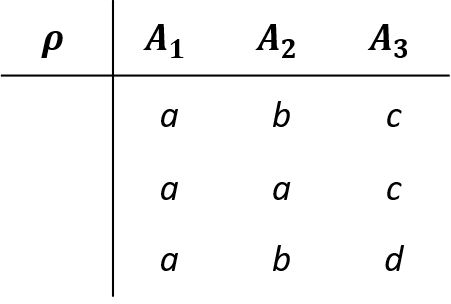
\includegraphics[width=0.3\linewidth]{1-1}
	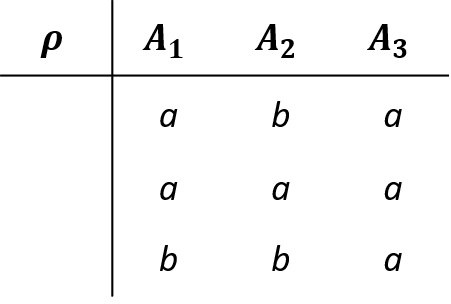
\includegraphics[width=0.3\linewidth]{1-1-2}
	\caption{Таблицы к примеру 1.5}
	\label{fig:1-1}
\end{figure}
\begin{question}
	Какое понятие более общее: отношение или функция ?
\end{question}
\begin{Remark}
	Понятие отношения и функции, или функциональной зависимости играет большую роль в теории баз данных.
\end{Remark}
Бинарные отношения допускают геометрическую интерпретацию!\\
$A=\{a,b,c \}$, пусть $\rho\subseteq A\times A$. Если на пересечении строки $i$ и столбца $j$ стоит $1$, то пара $(a_i,a_j)\in\rho$, если $0$, то $(a_i,a_j)\notin\rho$.\\
Возьмем на плоскости три кружка и обозначим их символами из $A$(рис. 3).
\begin{figure}[!htp]
	\centering
	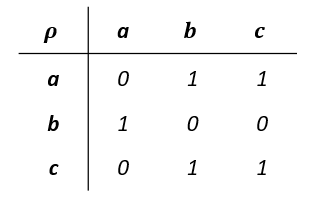
\includegraphics[width=0.3\linewidth]{1-2}
	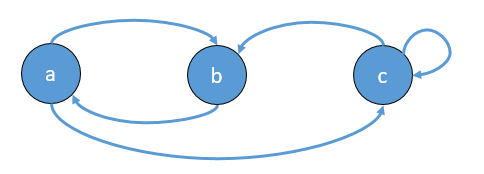
\includegraphics[width=0.3\linewidth]{1-3}
	\caption{Таблица и граф бинарного отношения}
\end{figure}
\begin{question}
	По какому правилу проведены стрелки?
\end{question}
Бинарное отношение называется:
\begin{enumerate}
	\item \textbf{рефлексивным}, если $(a_i,a_i)\in A_{\rho},\forall a_i\in A$.
	\item \textbf{симметричным}, если из $(a_i,a_i)\in A_{\rho}\Rightarrow(a_j,a_i)\in A_{\rho}$.
	\item \textbf{транзитивным}, если из $(a_i,a_j)\in A_{\rho}$ и $(a_j,a_k)\in A_{\rho}\Rightarrow (a_i,a_k)\in A_{\rho}$.
\end{enumerate}
\begin{question}
	Пусть $A=\{a_1,a_2,\ldots,a_n \}$. Как узнать, является ли бинарное отношение $A_{\rho}\in A\times A$: a) рефлексивным, б) симметричным, в) транзитивным?
\end{question}
В случае симметричного отношения вместо двух стрелок (ориентированных дуг) рисуют просто ребро (неориентированную дугу).
\begin{definition}
\textbf{Графом} $G$ называется пара множеств $G=(V,E)$, где $V=\{v_1,\ldots,v_n,\ldots \}$ - вершины графа и $E\subseteq V\times V=\{(v_{i_1},v_{j_1}),(v_{i_2},v_{j_2}),\ldots \}$ -ребра графа (пары вершин). 
\end{definition}
Если $|V|< +\infty$, то граф $G$ называется \textbf{конечным} (в противном случае - \textbf{бесконечным}). Если все ребра графа ориентированные, то и граф называется \textbf{ориентированным}(в противном случае граф называется \textbf{неориентированным}). Неориентированному графу $G=(V,E)$ всегда соответствует симметричное бинарное отношение $E\subseteq V\times V$. 
\begin{question}
	По графам бинарных отношений $\rho_1$ и $\rho_2$ построить их таблицы (матрицы)
\end{question}
\begin{figure}[!htp]
	\centering
	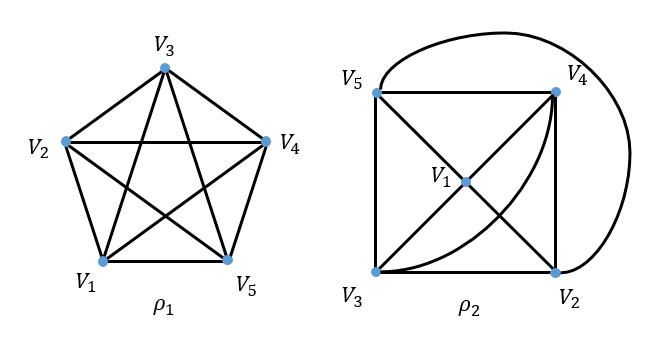
\includegraphics[width=0.5\linewidth]{1-4}
	\caption{К вопрос 1.5: Дуги пересекаются только в вершинах!}
	\label{fig:1-4}
\end{figure}
\begin{question}
	Сформулировать определение изоморфизма двух графов $G_1=(V_1,E_1), G_2=(V_2,E_2)$.
\end{question}
\begin{question}
	Какому отношению соответствует неориентированный граф?
\end{question}
\begin{figure}[!htp]
	\centering
	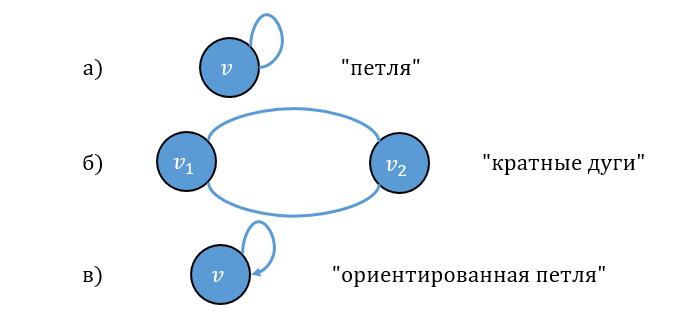
\includegraphics[width=0.6\linewidth]{1-5}
	\caption{К вопросу 1.7}
	\label{fig:1-5}
\end{figure}
Граф как отношение - нет кратных неориентированных ребер и неориентированных петель.\\
Граф как геометрический объект - может иметь кратные ребра, петли (в случае кратных ребер такой граф называют \textbf{мультиграфом}.) Мультиграф можно интерпретировать как отношение на \emph{расширенном} множестве $G=(V,E)$, где $E\subseteq (V\times V)\times\mathbb{N}$. То есть, каждому ребру присваивается число (номер ребра)
\begin{example}
$G_1=(\{v_1,v_2\}=V,\{(v_1,v_2,1),(v_1,v_2,2),(v_2,v_1,1),(v_2,v_1,2)\}=E).$
\begin{figure}[!htp]
	\centering
	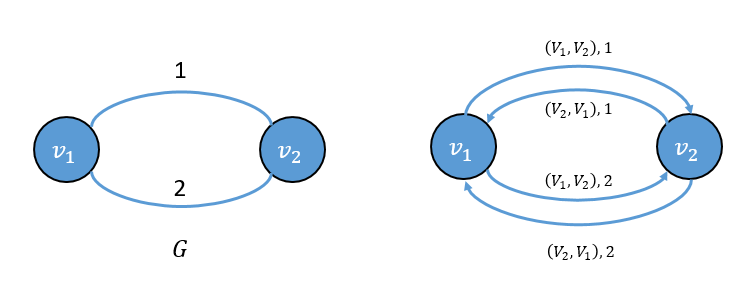
\includegraphics[width=0.6\linewidth]{1-6}
	\caption{Граф отношения}
	\label{fig:1-6}
\end{figure}
\end{example}
\section{Лекция 2}
Формальные системы $\Phi=\langle  X,F,A,R\rangle$.
\begin{itemize}
	\item $X$ - \textbf{алфавит} системы(список переменных)
	\item $F\subseteq X^*$ - выражения системы(\textbf{формулы} системы, атомарные(первичные) формулы системы). Формулы из $F$ задаются или списком или правилами их построения.
	\item $A\subseteq F$ - \textbf{аксиомы} системы(как правило соответствуют очевидным фактам предметной области)
	\item $R$ - \textbf{правила} вывода(правила получения новых формул).
\end{itemize}
\begin{example}
(Системы продукционного типа) $\Phi C_1$:
\begin{itemize}
	\item \textbf{Алфавит}: $X=\{x_1,\ldots,x_n \};|x|=n.$
	\item \textbf{Формулы}: $F=X^*$ - множество всех слов.
	\item \textbf{Аксиомы}: единственное выделенное слово $\tilde{\alpha_0}\in X^*$.
	\item \textbf{Правила вывода}: $\{R_i \}=\{\langle  \tilde{\beta}_1,\tilde{\beta}_2,\tilde{\beta}_3;\tilde{\beta}_1^{'},\tilde{\beta}_2^{'},\tilde{\beta}_3^{'}\rangle \}$.\\
	Если $ \alpha\in X^*$ имеет вид $\tilde{\alpha}=\tilde{\beta}_1\,\tilde{\delta}_1\,\tilde{\beta}_2\,\tilde{\delta}_2\,\tilde{\beta}_3\rightarrow \tilde{\beta}_1^{'}\,\tilde{\delta}_1^{'}\,\tilde{\beta}_2^{'}\,\tilde{\delta}_2^{'}\,\tilde{\beta}_3^{'}$- новое слово (формула).\\
	$"\rightarrow"$-"можно преобразовать".
\end{itemize}
\end{example}
Здесь $\tilde{\beta}_i ,\tilde{\beta}_i^{'},\tilde{\delta}_i ,\tilde{\delta}_i^{'},$- некоторое слова из $X^*,i=1,\ldots,3$. Некоторые из этих слов могут быть $\Lambda$.\\
\begin{equation*}
\tilde{\alpha}=\tilde{\beta}_1\,\tilde{\delta}_1\,\beta_2\,\tilde{\delta}_2\,\tilde{\beta}_3\rightarrow \tilde{\beta}_1^{'}\,\tilde{\delta}_1^{'}\,\tilde{\beta}_2^{'}\,\tilde{\delta}_2^{'}\,\tilde{\beta}_3^{'}
\end{equation*}
(\textbf{Подстановка}: слово $\tilde{\beta}_2$ заменяется на $\tilde{\beta}_2^{'}$).\\
$\Lambda\,\tilde{\delta}_1\,\tilde{\beta}_2\,\tilde{\delta}_2\,\Lambda\rightarrow \tilde{\delta}_1\,\tilde{\beta}_2^{'}\,\tilde{\delta}_2$ (\textbf{контекстная замена})\\
$\Lambda\,\tilde{\beta}_2\,\tilde{\delta}_2\,\Lambda\rightarrow \Lambda\,\tilde{\beta}_2\,\tilde{\delta}_2^{'}\,\Lambda$(\textbf{приписывание слова} $\beta_2^{'}$ (которое может быть равно $\beta_2$) в конец после слова $\delta_2 $. и т.д. Правил такого типа может быть много).\\
\underline{Выводимость} Слово $\tilde{\beta}$ \textbf{выводимо} из слова $\tilde{\alpha}$ в $\Phi C_1$, если существует такая цепочка
\begin{equation*}
\tilde{\alpha}\xrightarrow[R_{i_1}]{}\tilde{\gamma}_1\xrightarrow[R_{i_2}]{}\tilde{\gamma}_2\rightarrow\ldots\xrightarrow[R_{i_n}]{}\tilde{\gamma}_n=\tilde{\beta}
\end{equation*}
где $R_{i_1},R_{i_2},\ldots,R_{i_n } $ правила вывода(\textbf{продукции}) системы $\Phi C_1$. Число $n$ называется \textbf{длиной вывода} (слова $\tilde{\alpha} $ из $\tilde{\beta} $).
\begin{example}
	“Эволюция генотипа”\\
	$X=\{u,c,G,A\} $– алфавит.\\
	$\alpha_0$ аксиома: GA (генотип)\\
	правила вывода(эволюция геноьтипа):\\
	\begin{equation*}
	\begin{aligned}
	&\,\,R1.\quad\forall\widetilde{p}\in X^*,            \widetilde{p}\to\widetilde{p}\widetilde{p} \text{(удвоение или полиплодия)}\\
	&\left.
	\begin{matrix}
	R2.\quad\widetilde{p}AGA\widetilde{q}\to\widetilde{p}AA\widetilde{q}\\
	R3.\quad\widetilde{p}GAA\widetilde{q}\to\widetilde{p}AA\widetilde{q}
	\end{matrix}
	\right\}\text{ выпадение буквы (или } A \text{ делеция } \widetilde{p} \text{ и } \widetilde{q} \in X^*) (\text{могут быть } \Lambda!)
	\end{aligned}
	\end{equation*}
\textbf{Вывод (эволюция) из} $\widetilde{a}_0$\\
	$\alpha_0=GA\xrightarrow[R_1]{}G\underbrace{AGA}\xrightarrow[R_2]{} \underbrace{GAA}\xrightarrow[R_3]{}AA\xrightarrow[?]{} ...$\\
	$\alpha_0=GA\xrightarrow[R_1]{} GAGA\xrightarrow[R_1]{} G\underbrace{AGA}GAGA\xrightarrow[R_2]{}GA\underbrace{AGA}GA\xrightarrow[R_2]{}GAA\underbrace{AGA}\xrightarrow[R_2]{}\underbrace{GA}AAA\xrightarrow[R_3]{}AAAA\xrightarrow[R_2]{}$\\
	$\alpha_0=GA\xrightarrow[R_1]{}GA\underbrace{GA}\xrightarrow[R_1]{}GAGA\underbrace{GA}\xrightarrow[R_1]{}GAGAGAGA\xrightarrow[R_1]{}...$\\
\end{example}
Можно показать что любое слово (генотип) вида $(GA)^{n_1}(GA)^{n_2}...(GA)^{n_k}$\\
$(k\geq 1,n_k\in\mathbb{N})$ может появиться в процессе эволюции.\\
$(GA)^{n_i}=\underbrace{GAGA...GA}_{n_j \text{ раз}};A^i=\underbrace{A...A}_{i \text{ paз}}$.\\
Докажите это!\\
Никакое слово в котором есть комбинация $GG$ не может появиться.\\
Можно усложнить эту модель:\\
$R4.\quad$Если в слове $\widetilde{p}\in X^*$ \underline{два раза} появится комбинация $AA$ то этот генотип (потомок слова $\widetilde{a}_0$)\\
\underline{гибнет}: $\underbrace{\widetilde{p}_1 AA\widetilde{p}_2 AA}_{\widetilde{p}}\to\Lambda$.\\
Можно ввсти вместо "гибнет"  вероятность выживания:\\
Пусть появление $AA$ oзначает, что с вероятностью, например, $1/4$ он погибнет: $\widetilde{a}_0\to ... \underbrace{AA}_{1/4}\to ... \underbrace{AA}_{1/4}...\underbrace{AA}_{1/4}\to$.
\begin{question}
	Какая будет доля выживших потомков?(напрмер, длины n)
\end{question} 
\underline{Главная проблема}: По слову $\widetilde{p}\in X^*$ и набору правил $\{R_1,...,R_n\}$ понять, выводимо ли слово $\widetilde{p}$ из $\widetilde{a}_0$ с помощью правим (продукций) $R=\{R_1,...,R_n\}$. Иными словами $\widetilde{p}\in \big[X\big]^{\widetilde{a}_0}_R$!\\
Доказано,что в общем случае эта задача алогритмическим неразрешима!
\begin{example}\textbf{Задача на разрезание.}\\
Дано: Рисунки.\\
\begin{figure}[!htp]
	\centering
	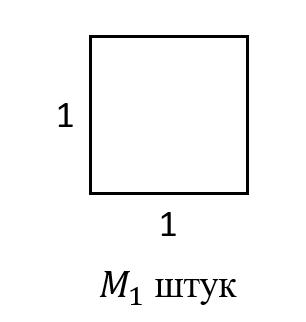
\includegraphics[width=0.2\linewidth]{2-1}
	\label{fig:2-1}
	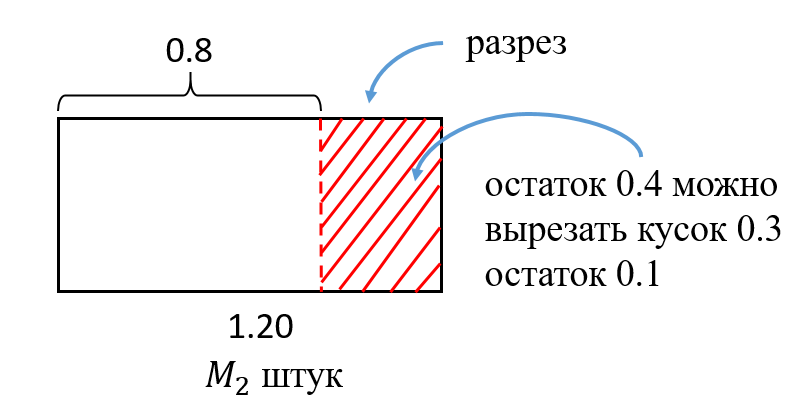
\includegraphics[width=0.5\linewidth]{2-2}
	\label{fig:2-2}
	\caption{К примеру 2.3}
\end{figure}
Надо: Получить (разрезать) так, чтобы: $n_1$ кусков $0.8$, $n_2$ кусков $0.6$, $n_3$ кусков $0.3$, и \underline{остакок был наименьшим}
\end{example}
Формализация задачи:\\
$\langle \underbrace{m_1,m_2}_{\text{количество кусков размера 1 и 1.20}};\underbrace{n_1,n_2,n_3}_{\text{количество кусков размера 0.8,0.6 и 0.3}}\rangle $\\
\\
\textbf{Акcиома} $\tilde{\alpha}_0 - \langle  M_1,M_2;0,0,0\rangle $\\
\textbf{Правила вывода}(продукции) $R$:\\
$R_1: \langle x+1,y;z,u,v\rangle \to \langle x,y;z+1,u,v\rangle $\\
$R_2: \langle x+1,y;z,u,v\rangle \to \langle x,y;z,u+1,v\rangle $\\
$R_3: \langle x+1,y;z,u,v\rangle \to \langle x,y;z,u+1,v+1\rangle $\\
$R_4: \langle x+1,y;z,u,v\rangle \to \langle x,y;z,u,v+3\rangle $\\
$R_5: \langle x,y+1;z,u,v\rangle \to \langle x,y;z+1,u,v+1\rangle $\\
$R_6: \langle x,y+1;z,u,v\rangle \to \langle x,y;z,u+2,v\rangle $\\
$R_7: \langle x,y+1;z,u,v\rangle \to \langle x,y;z,u+1,v+2\rangle $\\
$R_8: \langle x,y+1;z,u,v\rangle \to \langle x,y;z,u,v+4\rangle $\\
$R_9: \langle x,y+1;z,u,v\rangle \to \langle x,y;z+1,u,v+1\rangle $
\begin{question}
1.Одну продукцию можно удалить какую? - $R_2$\\
2.Что является в этой системе алфавитом $X$ и что есть $\widetilde{x}\in X^*$?
\end{question}
\begin{example}
	(преобразования слов)//
	$X=\{\text{А,Б,В,Г,...,Э,Ю,Я}\}$.\\
	$X^*=\{\text{любые конечные последовательности букв из X}\}$.\\
	\textbf{Аксиома}: $\alpha_0=$МАТР.\\
	\textbf{Правила}(продукции)\\
	$R_1: \forall \widetilde{x}\text{ и }\widetilde{\beta}\text{ из }X^*:\, \widetilde{x}\widetilde{\beta}\to\widetilde{\beta}\widetilde{x}$\\
	$R_2: \text{МАТ}\to\text{ТО}$\\
	$R_3: \text{РАС}\to\text{ТО}$\\
	$R_4: \text{Р}\to\text{РАС}$\\
	$R_5: \text{РАС}\to\text{РОС}$\\
	$R_6: \text{ТО}\to\text{АВ}$\\
	$R_7: \widetilde{x}T\widetilde{y}\to\widetilde{x}TT\widetilde{y}$(контексная замена)\\
	$\text{МАТР}\xrightarrow[R_4]{}\text{МАТРАС}\xrightarrow[R_3]{}\text{МАТТО}\xrightarrow[R_1]{}\text{ТОМАТ}$\\
	$\text{МАТР}\xrightarrow[R_1]{}\text{РМАТ}\xrightarrow[R_4]{}\text{РАСМАТ}\xrightarrow[R_5]{}\text{РОСМАТ}\xrightarrow[R_5]{}\text{МАТРОС}$
\end{example}
\begin{question}
	Можно ли из МАТР получить АВТОМАТ используя $R_1-R_8$ и как?
\end{question}
\begin{example}
	$X=\{\text{М,А,П}\}$   $R_1:\text{М}\to\text{П}$   $R_2:\text{П}\to\text{М}$\\
	аксиома - слово ПАПА: $\text{ПАПА}\xrightarrow[R_2]{}\text{МАПА}\xrightarrow[R_2]{}\text{МАМА}\xrightarrow[R_1]{}\text{ПАМА}\xrightarrow[R_1]{}\text{ПАПА}\xrightarrow[...]{}...$\\
	аксиома $AA\xrightarrow[?]{}$\\
	аксиома АП: $\text{АП}\to\text{АМ}\to\text{АП}\to\text{АМ}\to\text{АП}\to...$
\end{example}
\begin{example}
$X=\{\text{М,А,П}\}$\\
Правила R: $\text{М}\to\text{П}$, $\text{А}\to\text{П}$, $\text{М}\to\text{А}$, $\text{П}\to\text{М}$, $\text{А}\to\text{М}$, $\text{П}\to\text{А}$.
\end{example}
\begin{question}
	что содержит $\big[X\big]^{\widetilde{a}_0}_R$?
\end{question}
$\big[X\big]^{\widetilde{a}_0}_R$ - множество всех слов, которые получаются из $\alpha_0\in X^*$ применением правил вывода $R$. Это множество называется \underline{\text{замыканием}} $X$ относительно слова $\widetilde{a}_0$ и правила $R$.
\begin{example}
$X=\{\text{М,А,П}\}$\\
К правилам $R$ из предыдущего примера добавалено правило $R_1:A\to AA$
\end{example}
\begin{question}
Отличается ли $\big[X\big]^{\widetilde{a}_0}_{R\cup R_1}$ от $\big[X\big]^{\widetilde{a}_0}_R$ ? Если да, то чем?
\end{question}


\section{Лекция 3}
Исчисление высказываний (calculus of propositions) \\
\textbf{высказывание} - любое предложения языка(русского, английского,греческого...), про которое можно сказать \textbf{истинно(True)} оно или \textbf{ложно(False)}.
\begin{example}
	1. ``Все студенты - отличники''.\\
	2. ``В десятичной системе $2\times 2=4$''.\\
	3. ``В невырожденном треугольнике сумма двух сторон больше третьей стороны''.\\
	4. ``Луна состоит из зелёного сыра''.\\
	5. ``Вода не может прератиться в лёд''.\\
	6. ``Идёт дождь''.\\
	7. ``Ручка упала на пол''.\\
	Предложения 1,2,3,4,5 - высказывания; 1,2,3 - истинные, 4,5 - ложные.\\
	Предложения 6,7 - не высказывания - они ни истинны и не ложны.
\end{example}
Будем обозначать предложения высказывания символами $\{P_1,P_2,...,P_n,...\}$ - это пропозицииональные переменные. Поскольку смысл(sense) высказываний нас не нитересует(важно истинно высказывание или ложно) то можно считать, что $P_1,...,P_n,...$ - \textbf{булевские переменные} и принимают значение ``0''(если высказывание ложно) и ``1''(если высказывание истинно).\\
Из высказываний с помощью связок ``и'', ``или'', ``не'', ``если A то B'', ``$\land$'', ``$\lor$'', ``$\lnot$,-'', ``$A\supset B$'' и т.д. можно строить более \textbf{сложные высказывания}.\\
Истинно сложное высказывание или нет зависит от истинности или ложности входящих в него высказываний и от множества используемых связок.\\
Нам пока достаточно будет двух связок $``\lnot''$ - не (или отрицание) и ``$A\supset B$''(если A то B).\\
$\Phi C_{\text{ИВ}}:$
\begin{itemize}
	\item \textbf{Алфавит системы}\\ 
	$X=\{(,),\lnot,\supset,P_1,P_2,...,P_n,...\}$.
	\item \textbf{Формулы $F$}\\
	1)$(P_1),(P_2),...,(P_n),...$ - формулы(элементраные формулы).\\
	2)Если A - формула, то $(\lnot A)$ тоже формула.\\
	3)Если A и B - формула, то $(A\supset B)$ тоже формула.\\
	4)Других формул нет.
	\item \textbf{Аксиомы системы}\\
	$A_1.(A\supset (B\supset A))$.\\
	$A_2.((\lnot B\supset \lnot A)\supset (A\supset B))$.\\
	$A_3.(A\supset (B\supset C))\supset ((A\supset B)\supset (A\supset C))$.\\
	- Это схема аксиом.
	\item \textbf{Правила вывода}\\
	$R_1$. Вместо формул \underline{A и B} разрешаться подставлять \underline{любые формула} F полученные по пунктам 1-4.\\
	$R_2$. Если у нас есть формулы A и $A\supset B$, то тогда есть и формула B.\\
	$R_1$. - правило подстановки.\\
	$R_2$. - правило отделения формулы(modus ponens).\\
\end{itemize}
\begin{example}
	$A_1: A\supset (B\supset A)$ - аксиома.\\
	$A\supset (A\supset A)$ - тоже аксиома.\\
	$A\supset((A\supset A)\supset A)$ - тоже аксиома.\\
	...\\
	смотри правило $R_1$.\\
	\\
	Правило $R_2$:\\
	$A,A\supset B$, то есть формула B.\\
	A - $\underbrace{\text{``квадрат четного числа''}}_{\text{высказывание}}$.\\
	B - ``квадрат четного числа делится на 4''.\\
	$A,A\supset B$ - ``квадрат четного числа'' если ``квадрат четного числа'' то ``квадрат четного числа делится на 4''.\\
	Мы из A и $A\supset B$ получил B.
\end{example}
Нас интересует в этой ``игре в формулы''.
\begin{question}
	$[F]_{R_1,R_2} = ?$ - то есть какие формулы можно получить из аксиом $A_1-A_3$ используя правила вывода $R_1,R_2$.\\
	Докажем, что формула $(A\supset A)\in [F]_{R_1,R_2}$. Все формулы над $\{\lnot,\supset\}$. Верно ли что $F=[F]_{R_1,R_2}$?\\
	\begin{figure}[!htpb]
	\centering
	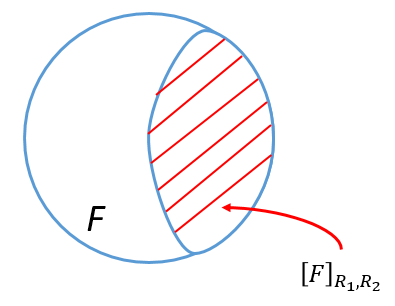
\includegraphics[width=0.3\linewidth]{3-1}
	\caption{К вопросу 3.1}
	\label{fig:3-1}
\end{figure}
\end{question}
	Покажем, что формула $(A\supset A)\in [F]_{R_1,R_2}$ для $\forall A\in F$.\\
	1. $(A\supset (\underbrace{B}_{A\supset A \text{ правило } R_1}\supset A))$ - аксиома $A_1$\\
	$(A\supset ((A\supset A)\supset A))$\\
	2. $(A\supset (\underbrace{B}_{A\supset A}\supset \underbrace{C}_{A \text{ правило } R_1}) )\supset ((A\supset B)\supset (A\supset C))$ аксиома $A_2$\\
	$(A\supset ((A\supset A)\supset A))\supset (A\supset (A\supset A))\supset (A\supset A)$\\
	Из 1 и 2 по правилу $R_2$ (т.р.) $(A\supset (A\supset A))\supset (A\supset A)$.\\
	3. $(A\supset (\underbrace{B}_{A \text{ правило } R_1}\supset A))$ - аксиома $A_1$.\\
	$(A\supset (A\supset A))$\\
	4. Из 2 и 3 по правилу $R_2,(A\supset A)$ то есть $\forall A\in F$ формула $(A\supset A)$ выводима, то есть $\in[F]_{R_1,R_2}$.\\
	Напоминание: 
	\begin{figure}[!htpb]
	\centering
	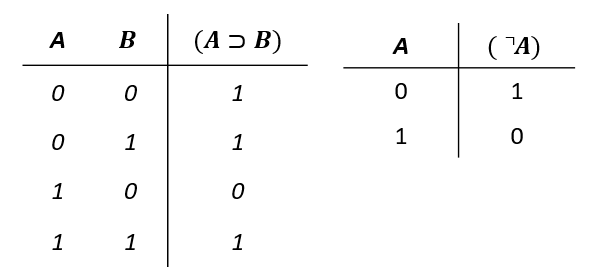
\includegraphics[width=0.5\linewidth]{3-2}
	\caption{Напоминание!}
	\label{fig:3-2}
\end{figure}
	Зная эти таблициы мы можем определить заначение (истинна или ложна) любой формулы из F.\\

\begin{example}
	1. $A\supset (A\supset A)$.	2. $(A\supset A)\supset A$.\\
	\begin{figure}[!htp]
		\centering
		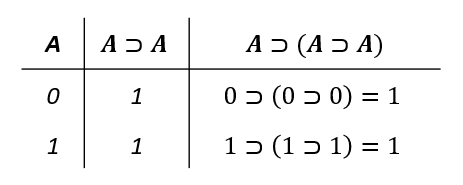
\includegraphics[width=0.4\linewidth]{3-3}
		\label{fig:3-3}
		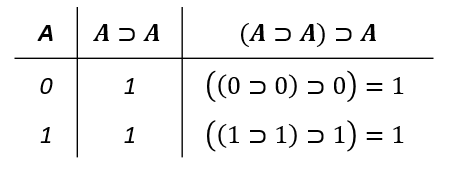
\includegraphics[width=0.4\linewidth]{3-4}
		\label{fig:3-4}
		\caption{К примеру 3.3}
	\end{figure}	
	Расстановка скобок играет роль!
\end{example}
\begin{definition}
Формула $\Phi(A_1,...,A_n)$ называется:\\
	1) $\equiv 0$ (тождественно ложной) если при $\forall$ наборе значений формул $A_1,A_2,...,A_n, \Phi\equiv 0$ (\textbf{не выполнимые} формулы).\\
	2) $\equiv 1$ (тождественно истинная) если при $\forall$ наборе значений формул $A_1,A_2,...,A_n, \Phi\equiv 1$ (\textbf{тавтологии} или \textbf{общезнанимая} формула).\\
	3) \textbf{Выполнимой} если на некоторых наборах значений формула $A_1,A_2,...,A_n$. Она принимает $\Phi\equiv 1$, а на остальных $\Phi\equiv 0$.
\end{definition}
	Заметим, что $A\supset A\equiv A\lor \bar{A}\equiv 1$ \underline{закон ``исключенного третьего''!}
\begin{theorem}
    \label{theorem 2-1}
	$\forall$ формула $\in [F]_{R_1,R_2}$ является тавтологей.
\end{theorem}
Прежде чем доказывать вспомним из круса ``дискретной математики''.\\
\begin{figure}[!htpb]
	\centering
	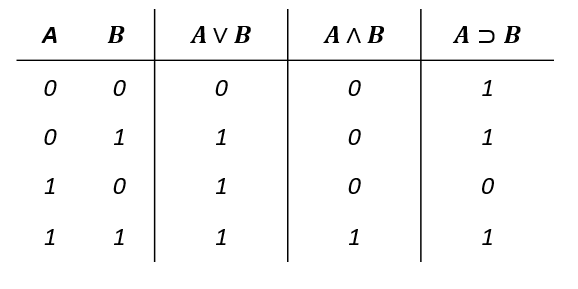
\includegraphics[width=0.4\linewidth]{3-5}
	\caption{Вспомним из курса ДМ}
	\label{fig:3-5}
\end{figure}
По этим таблицам легко проверить, что:\\
$A\supset B\equiv \bar{A}\lor B\Rightarrow \left\{\begin{array}{cc}
{A\lor B}\equiv \bar{A}\supset B \quad (1)\\
{A\land B}\equiv \overline{A\supset \bar{B}} \quad (2)\\
A\lor \bar{A}\equiv 1
\end{array}\right.$ 

Поэтому мы далее можем испосльзовать операцию дизъюнкции($\lor$) и конъюнкции($\land$), понимая их как формулы (1) и (2). ``-'' - знак операции отрицания. - Будем его использовать тоже.\\
\emph{Доказательство} теоремы 3.1:\\
1. Докажем, что аксиомы являются тавтологиями.\\
$A\supset(B\supset A)=A\supset (\bar{B}\lor A)=\bar{A}\lor (\bar{B}\lor A)=(\bar{A} \lor A) \lor \bar{B}=1\lor \bar{B}\equiv 1$.\\
2. $(\lnot B\supset \lnot A)\supset ((\lnot B\supset A)\supset B)=(B\lor \bar{A})\supset ((B\lor A)\supset B)=\overline{(B\lor \bar{A})}\lor \overline{B\lor A}\lor B=(\bar{B}\land \bar{A})\lor (\bar{B}\land A)\lor B=\bar{B}(\underbrace{\bar{A}\lor A}_{=1})\lor B=\bar{B}\lor B\equiv 1$.\\
3. $(A\supset (B\supset C))\supset ((A\supset B)\supset (A\supset C))\equiv 1$. Самостоятельно !\\
Можно было бы построить таблицу и проверить по ней значения формул.
\begin{figure}[!htpb]
	\centering
	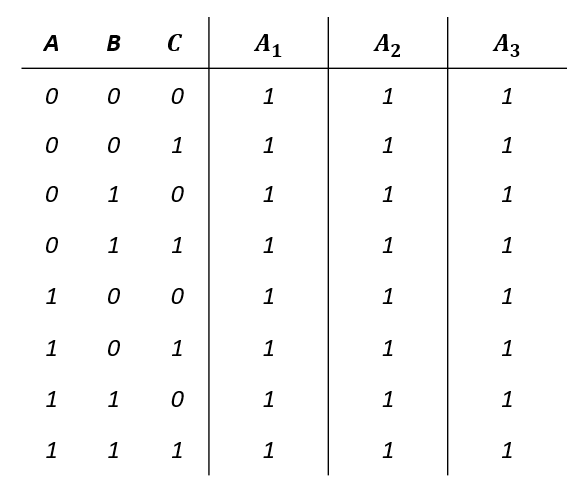
\includegraphics[width=0.5\linewidth]{3-6}
	\caption{Таблица к доказательству теоремы}
	\label{fig:3-6}
\end{figure}
То есть аксиомы $A_1,A_2,A_3$ являются тавтологиями (для любых формул $A,B,C$ из $F$). \\
Заметим, что если $A$ и $A\supset B$ тавтологии, то $B$ тоже тавтоголия. Если это не так, то при некотором наборе значений подформул, входящих в $B$, она будет $=0$, но $A=1$ при этом распределении значений истинности ($A=1$, тавтология !) Получаем $(A\supset B)\Rightarrow (1\supset 0)=0,$ т.е. $(A\supset B)\ne 1$. (не тавтология ) - Противоречие. Теорема доказана.\\
И так, мы доказали теорему 1. (Смысл: если формула $\Phi$ из $F$ выводима из аксиом $A_1 - A_3$ правилами вывода $R_1,R_2$, то $\Phi\equiv 1$($\Phi$ - тавтология)).
\begin{theorem}
	\label{theorem 2-2}
	Если $\Phi\equiv 1$, то она принадлежит $\big[F\big]_{R_1,R_2}$.
\end{theorem}
Доказывается в любом стандартном курсе ``Математическая логика''.\\
Объединяя теорему \ref{theorem 2-1} и \ref{theorem 2-2} получаем
\begin{theorem}
	(о полноте исчисления высказываний)\\
	Формула $\Phi$ исчисления высказываний принадлежит $\big[F\big]_{R_1,R_2}\Leftrightarrow \Phi \equiv 1$. Иными словами: $\Phi\in \big[F\big]_{R_1,R_2}\Leftrightarrow \Phi \equiv 1$(т.е. общезначима!)
\end{theorem}
\begin{definition}
	(логического следствия)\\
	Формула $\Phi$ является \textbf{логическим следствием} формул $\Phi_1,\ldots,\Phi_n$, если из $\Phi_1,\ldots,\Phi_n=1$ следует, что и $\Phi=1$. Т есть если $\Phi_1\wedge\ldots\wedge \Phi_n=1,$ то и $\Phi=1$.
\end{definition}
\begin{proposition}
	$\Phi$ является логическим следствием $\Phi_1,\ldots,\Phi_n\Leftrightarrow$ формула ($\Phi_1\wedge\ldots\wedge \Phi_n\supset \Phi$)$\equiv 1$(т.е. общезначима).
\end{proposition}
\emph{Доказательство}\\
\emph{Достаточность.} Пусть $\Phi$ - логическое следствие $\Phi_1,\ldots,\Phi_n$, т.е. если $\Phi_1\wedge\ldots\wedge \Phi_n=1$, то $\Phi=1$; если $\Phi_1\wedge\ldots\wedge \Phi_n=0$, то $0\supset \Phi=1$( по определению $\supset$.) Случая $\underbrace{\Phi_1\wedge\ldots\wedge \Phi_n}_{=1}\supset\underbrace{\Phi}_{=0}$ быть не может, т.к. $\Phi$ - логическое следствие $\Phi_1,\ldots,\Phi_n$. Следовательно $((\Phi_1\wedge\ldots\wedge \Phi_n)\supset \Phi)\equiv 1$.\\
\emph{Необходимость.} Пусть $((\Phi_1\wedge\ldots\wedge \Phi_n)\supset \Phi)\equiv 1$. Значит если $\Phi_1\wedge\ldots\wedge \Phi_n=1$, то и $\Phi=1$. В противном случае $\Phi_1\wedge\ldots\wedge \Phi_n=1$, а $\Phi=0\Rightarrow (\Phi_1\wedge\ldots\wedge \Phi_n)\supset \Phi)=0$ - т.е. $(\Phi_1\wedge\ldots\wedge \Phi_n\supset \Phi)$ - не общезначима. - Противоречие. \hfill $\qedsymbol$ \\
\\
Пусть $I^1_{\Phi}$ - множество наборов значений всех переменных, входящих в $\Phi$, на которых $\Phi=1$. Тогда если $\Phi$ - логическое следствие $\Phi_1\wedge\ldots\wedge \Phi_n$, то $I^1_{\Phi}\subseteq I^1_{\Phi_1\wedge\ldots\wedge\Phi_n}$.
\begin{definition}
Пусть $\Phi=\Phi(\rho_1,\ldots,\rho_n)$. Любой набор значений переменных $(\rho_1,\ldots,\rho_n)\in E^n_2=E_2\times\ldots\times E_2$ ($E_2=\{0,1\}$) называется \textbf{интерпретацией формулы} $\Phi$. Множество всех интерпретаций $\Phi$, где $\Phi=1$, называется \textbf{моделью} для $\Phi$.
\end{definition}
 Т.е. если $\Phi$ - общезначима, то $\{I^1_{\Phi} \}=E^n_2$, если $\Phi$ невыполнима, то $\{I^1_{\Phi}\}=\Phi$, если $\Phi$ - выполнима, то $\{I^1_{\Phi} \}=A\subset E^n_2 $ и $A\ne0$.
\begin{proposition}
	Формула $(\Phi_1\wedge\ldots\wedge\Phi_n\supset\Phi)$ общезначима $\Leftrightarrow(\Phi_1\wedge\ldots\wedge\Phi_n\wedge\bar{\Phi})$ - невыполнима. 
\end{proposition}
\begin{definition}
Если из $M_1\models B_1,M_1\models B_2,\ldots,M_1\models B_s$, то говорим, что множество формул $M_2=\{B_1,\ldots,B_s \}$ \textbf{выводимо} из множества формул $M_1$(обозначение $M_1\models M_2$).
\end{definition}
\begin{proposition}
	Если $M_1\models M_2,M_2\models M_3$, то $M_1\models M_3$.
\end{proposition}
Доказательство самостоятельно !\\
Теперь у нас есть процесс построения модели ПО:
\begin{figure}[!htbp]
	\centering
	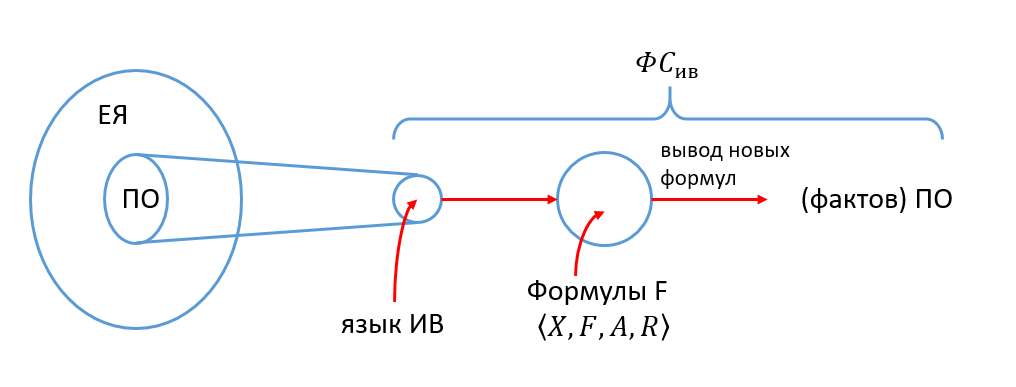
\includegraphics[width=0.7\linewidth]{3-7}
	\caption{Процесс построения модели ПО}
	\label{fig:3-7}
\end{figure}
Здесь $A$ - аксиомы - очевидные высказывания о ПО. Мы можем задать вопрос так: верно ли что из фактов $\Phi_1,\ldots,\Phi_n$ следует $\Phi$? Для этого (как мы показали выше) надо доказать, что формула $(\Phi_1\wedge\ldots\wedge \Phi_n\supset \Phi)\equiv 1$ или $(\Phi_1\wedge\ldots\wedge\Phi_n\wedge\bar{\Phi})\equiv 0$.\\
\emph{Доказательство}.\\
 Пусть $(\Phi_1\wedge\ldots\wedge\Phi_n\supset\Phi)\equiv 1$$\Leftrightarrow \overline{(\Phi_1\wedge\ldots\wedge\Phi_n\supset\Phi)}\equiv \bar{1}\equiv 0$$\Leftrightarrow \overline{(\overline{(\Phi_1\wedge\ldots\wedge\Phi_n)}\vee\Phi)}\equiv 0$\\
$\Leftrightarrow \overline{\overline{(\Phi_1,\ldots,\Phi_n)}}\wedge \bar{\Phi}\equiv 0$ $\Leftrightarrow(\Phi_1,\ldots,\Phi_n)\wedge \bar{\Phi}\equiv 0$.
\begin{question}
	Какие булевские тождества здесь были использованы?
\end{question}
Пусть $M=\{\Phi_1,\ldots,\Phi_n \}\subseteq F$ - некоторое множество формул. Говорим, что формула $\Phi$ \textbf{выводима} из $M$ (обозначение $M\models$), если формула $\Phi_1\wedge\ldots\wedge\Phi_n\supset \Phi$ общезначима.
\begin{proposition}
1) Если $M\models A_1$ и $M\models A_2$, то $M=A_1\wedge A_2$.\\
2) Если $M_1\models A_1$ и $M_2\models A_2$, то $M_1\wedge M_2\models A_1\wedge A_2$.\\
3) Если $M\models A_1\wedge A_2$, то $M\models A_1$ и $M\models A_2$.
\end{proposition} 
Доказать самостоятельно!
\begin{example}
\textbf{Моделирование химических реакций}\\
1. $Na+Cl_2\to NaCl$\\
2. $CH_4+O_2\to CO_2+H_2O$\\
... и так далее
\end{example}
Обозначим $Na\,-\,\Phi_1,Cl_2\,-\,\Phi_2,NaCl\,-\,\Phi_3$, тогда реакцию 1. можно записать как $\Phi_1\wedge \Phi_2\supset \Phi_3$. $CH_4\,-\,\Phi_1,O_2\,-\,\Phi_2,CO_2\,-\,\Phi_3,H_2O\,-\,\Phi_4$, реакцию 2. можно записать как $\Phi_1\wedge \Phi_2\supset \Phi_3\wedge \Phi_4$. Таким образом, аксиомы (они же и элементарные формулы) - это правила вывода.
\begin{question}
\underline{Задача.} Есть база фактов (база данных) БД$=\{\Phi_1,\Phi_2,\Phi_3,\Phi_4 \}$ - какие-то вещества. \\
Есть база правил (база знаний) - химические реакции. БЗ$=\{\Phi_1\wedge\Phi_2\supset \Phi_5\wedge\Phi_6,\Phi_5\wedge\Phi_3\supset \Phi_7\wedge\Phi_2,\Phi_7\wedge\Phi_4\supset \Phi_8\wedge\Phi_{10},\Phi_8\wedge\Phi_9\supset \Phi_1\}$.\\
Можно ли получить вещество $\Phi_9$?
\end{question}
Для ответа нада доказать, что $\Phi(\Phi_1,\Phi_2,\ldots,\Phi_{10})=((\Phi_1\wedge \Phi_2\supset \Phi_3\wedge \Phi_4)\wedge(\Phi_1\wedge\Phi_2\supset \Phi_5\wedge\Phi_6)\wedge(\Phi_5\wedge\Phi_3\supset \Phi_7\wedge\Phi_2)\wedge(\Phi_7\wedge\Phi_4\supset \Phi_8\wedge\Phi_{10})\wedge(\Phi_8\wedge\Phi_9\supset \Phi_1))\supset \Phi_9\equiv 1$.\\
Если строить таблицу, то в ней будет $2^{10}=1024$ бинарных строк длины $10$. Как проверять общезначимость?
\begin{enumerate}
	\item табличный способ
	\item метод эквивалентных преобразований
	\item метод резолюций и его варианты
	\item эвристические методы
\end{enumerate}
\begin{Remark}
	(о химии реакциях)\\
	$2Na+2H_2O\to 2NaOH+H_2$\\
	$2NaOH+SiO_2\to Na_2SiO_3+H_2O$\\
	$Na_2Si_3O_3+2HCl\to 2NaCl+H_2SiO_3$\\
	$2NaCl\to 2Na+Cl_2$
\end{Remark}
\section{Лекция 4}
Рассмотрим формулу $\Phi=(\underbrace{(P_1\wedge P_2)\supset P_3)}_{\Phi_1}\wedge(\underbrace{(P_4\wedge P_3)}_{\Phi_2}\supset\underbrace{(P_5\wedge P_1)}_{\Phi_3})$.
\begin{question}
Определить, к какому классу относится $\Phi$:\\
1. общезначимых $(\equiv 1)$,\\
2. невыполнимых $(\equiv 0)$,\\
3. выполнимых ($=1$ на части наборов значений переменных и $=0$ на другой части) 
\end{question}
\noindent\textbf{1. Проверка по таблице}\\
\begin{figure}[!htbp]
	\centering
	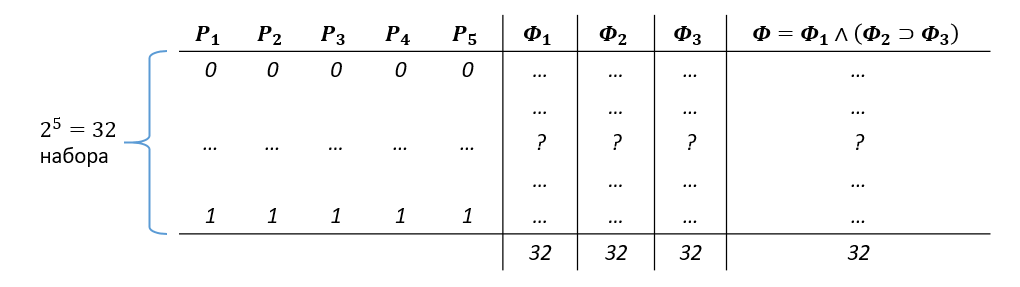
\includegraphics[width=0.9\linewidth]{4-1}
	\caption{Проверка по таблице}
	\label{fig:4-1}
\end{figure}
\textbf{2. Метод Квайна(семантические деревья)}\\
\begin{figure}[!htbp]
	\centering
	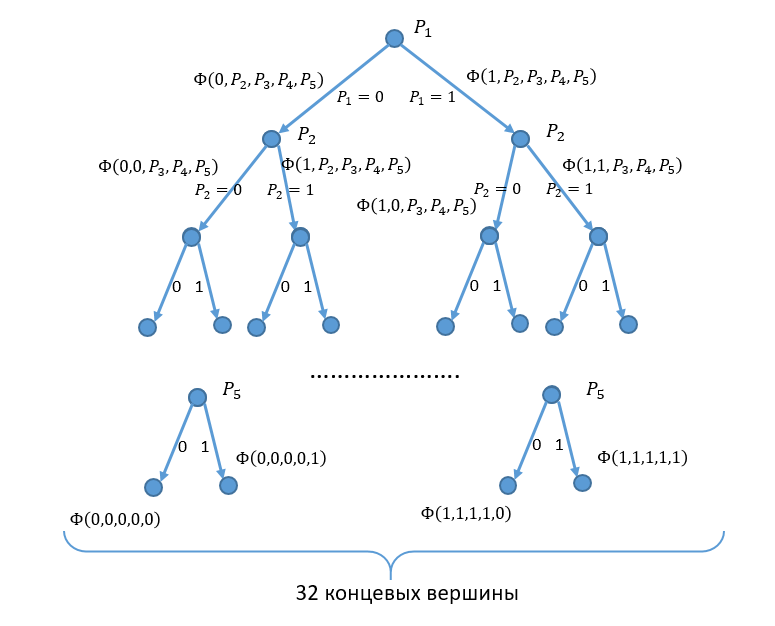
\includegraphics[width=0.9\linewidth]{4-2}
	\caption{Метод Квайна-1}
	\label{fig:4-2}
	\centering
	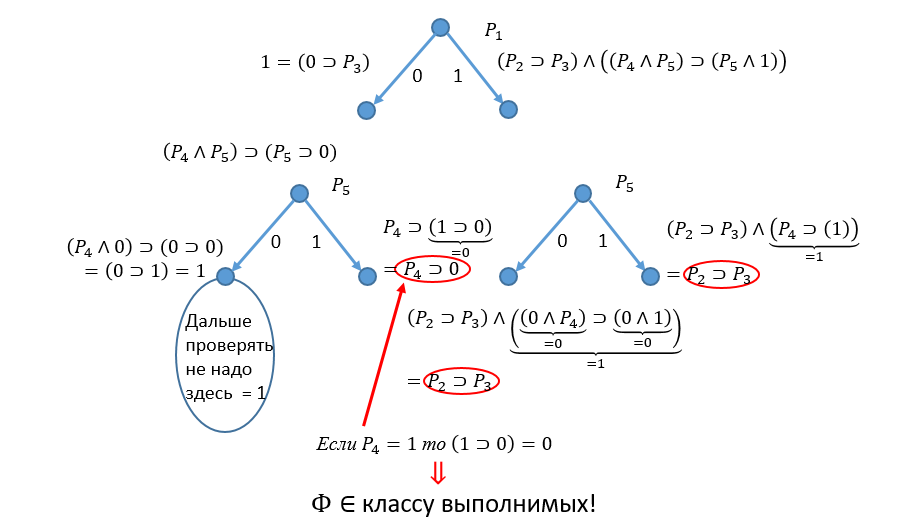
\includegraphics[width=0.9\linewidth]{4-3}
	\caption{Метод Квайна-2}
	\label{fig:4-3}
\end{figure}
Если на всех $32$ концевых вершинах $\Phi=1$, то она общезначима(тавтология); если $\Phi=0$, то она невыполнима; если есть $\Phi(\alpha_1,\ldots,\alpha_5)=1$ и $\Phi(\beta_1,\ldots\beta_5)=0$, то она выполнима.\\
\underline{Важно:} Порядок выбора переменных существенен: принадлежность $\Phi$ к классам $1-3$ можно обнаружить раньше (не перебирая) \underline{все} варианты. Рассмотрим формулу $\Phi$ (начало лекции): $\Phi=((P_1\wedge P_2)\supset P_3)\wedge((P_4\wedge P_3)\supset(P_5\wedge P_1))$.(см. рис. метод Квайна-2)\\
\textbf{3. Метод эквивалентных преобразований}\\
В дискретной математике приводится система тождеств
\begin{itemize}
	\item  Коммутативность $\vee$ и $\wedge$:\\
	$x_1\vee x_2\equiv x_2\vee x_1,$\\
	$x_1\wedge x_2\equiv x_2\wedge x_1$.
	\item Ассоциативность $\vee$ и $\wedge$:\\
	$(x_1\vee x_2)\vee x_3\equiv x_1\vee (x_2\vee x_3),$\\
	$(x_1\wedge x_2)\wedge x_3\equiv x_1\wedge (x_2\wedge x_3).$
	\item Дистрибутивность $\wedge$ относительно $\vee$ и наоборот:\\
	$x_1\vee (x_2\wedge x_3)\equiv (x_1\vee x_2)\wedge(x_1\vee x_3),$\\
	$x_1\wedge (x_2\vee x_3)\equiv (x_1\wedge x_2)\vee(x_1\wedge x_3).$
	\item Правила Моргана:\\
	$\overline{\bar{x}_1\vee \bar{x}_2}\equiv x_1\wedge x_2$,\\
	$\overline{\bar{x}_1\wedge \bar{x}_2}\equiv x_1\vee x_2$.
	\item Правило снятия двойного отрицания:\\
	$\bar{\bar{x}}\equiv x$.
	\item $x\vee 1\equiv 1\quad x\wedge 1\equiv x$\\
	$x\vee 0\equiv x\quad x\wedge 0\equiv 0$\\
	$x\vee \bar{x}\equiv 1\quad x\wedge \bar{x}\equiv 0$\\
	$x\vee\bar{x}\equiv x\quad x\wedge x\equiv x$
\end{itemize} 
	В курсе ``дискретной математики'' про систему 1-6 доказывают, что она обладает свойством синтаксической полноты, то есть для любых двух формул( $\Phi=\{\land,\lor,-\}$) за конечиное число шагов(эквивалентных преобразований) можно выяснить эквивалентны формулы или нет.
	\begin{example}
		$\Phi_1=x,  \Phi_2=(x\land y)\lor (x\land \bar{y})$\\
		$\Phi_1=x \underbrace{\Rightarrow}_{x\land 1\equiv x} x\land 1 \underbrace{\Rightarrow}_{y\lor \bar{y}\equiv 1}x\land(y\lor \bar{y})\underbrace{\Rightarrow}_{\text{дистриб.}} (x\land y)\lor (x\land \bar{y})$;\\
		То есть формулы $\Phi_1 \backsim \Phi_2$ (``$\backsim$'' - эквивалентность из 3).\\
		$\Phi_2$ выводится из $\Phi_1$ с помощью тождеств 1-6 если есть цепочка подстановок $\Phi_1\underbrace{\Rightarrow}_{R_{i_1}}\Phi_1^{'} \underbrace{\Rightarrow}_{R_{i_2}}...\underbrace{\Rightarrow}_{R_{i_s}}\Phi_S^{'}  =\Phi_2$. Здесь $R_{i_1},...,R_{i_s}$ взяты из 1-6.\\
	 	Подстановка в формулу: $\Phi =(...,\Phi_1 ,...)\Rightarrow \Phi^{'} =\Phi(...,\Phi_2 ,...)$ если есть тождество $\Phi_1\equiv \Phi_2$.\\
	 	Если с помощью тождественных преобразований удается показать, что $\Phi\equiv 1 (\Phi \equiv 0)$ то $\Phi$ - общезначаем(невыполнима) в остальных случаях $\Phi$ - выполнима.
	\end{example}
	\begin{Remark}
		$x\supset y \equiv \bar{x}\lor y,$\quad$x\lor y \equiv \bar{x}\supset y,$\quad$x\land y \equiv \overline{x\supset \bar{y}}$.
	\end{Remark}
	То есть, любое сложное высказывание построенное с помощью связок $\{\land ,\lor ,-\}$ можно преобразовать в эквивалентное ему высказывание с использованием $\{\supset ,-\}$ и наоборот.
	\begin{example}
		Вместо $x\land y$ будем писать просто $xy$.\\
		1. $\Phi_1 = \bar{x}\bar{y}\lor \bm{xy \lor \bar{x}y}\lor x\bar{y}\underbrace{\Rightarrow}_{\text{коммут. }\lor} \bar{x}\bar{y}\lor \bar{x}y\lor xy\lor x\bar{y}\underbrace{\Rightarrow}_{\text{диcтриб.}}\bar{x}\underbrace{(\bar{y}\lor y)}_{\bar{y}\lor y\equiv 1}\lor xy \lor x\bar{y}\Rightarrow \underbrace{\bar{x}\cdot 1}_{\bar{x}\cdot 1=\bar{x}}\lor xy\lor x\bar{y}\underbrace{\Rightarrow}_{\text{диcтриб.}}\bar{x}\lor x\underbrace{(y\lor \bar{y})}_{y\lor \bar{y}=1}\Rightarrow \bar{x}\lor x\cdot 1=\bar{x}\lor x\equiv 1$.\\
		Формула $\Phi_1\equiv 1$, т.е. тавтология.\\
		2.$(x\supset \bar{y})\land (y\supset x)\land (y\supset y)\Rightarrow (\bar{x}\lor \bar{y})\land (\bar{y}\lor x)\land (\bar{y}\lor y)\Rightarrow \bar{x}\land (\bar{y}\land x)\lor \bar{y}\land (\bar{y}\lor x)\land 1\Rightarrow \bar{x}\bar{y}\lor \underbrace{\bar{x}x}_{=0}\lor \underbrace{\bar{y}\bar{y}}_{=0}\lor \bar{y}x\Rightarrow \bar{x}\bar{y}\lor \bar{y}x \Rightarrow \bar{y}\underbrace{(x\lor \bar{x})}_{=1}\Rightarrow \bar{y}$ - выполнима (1) $y=0$ то $\bar{y}=1$.(2) $y=1$ то $\bar{y}=0$.\\
		3. $\underbrace{(x\lor y)(\bar{x}\lor y)}_{=(\underbrace{x\bar{x}}_{=0}\lor xy\lor y\bar{x}\lor \underbrace{yy}_{=y})}\wedge\underbrace{(x\lor \bar{y})(\bar{x}\lor \bar{y})}_{=\underbrace{(x\bar{x}}_{=0}\lor x\bar{y}\lor \bar{y}\bar{x}\lor \underbrace{\bar{y}\bar{y})}_{\bar{y}}}=(xy\lor y\bar{x}\lor y)(x\bar{y}\lor \bar{y}\bar{x}\lor \bar{y})=(y\underbrace{(x\lor \bar{x}\lor 1}_{=1}))(\underbrace{x\lor \bar{x}}_{=1}\lor 1)\bar{y}=y\cdot \bar{y}\equiv 0$. Формула невыполнима.\\
		Трудности реализации на компьютер = Наиболее удобные для программирования метод - резолюция.\\
	\end{example}
\textbf{Метод резолюций в} $\Phi C_\text{ИВ}$.\\
Далее мы будем рассматривать формулы специального вида:\\
Формула $L$ называется \textbf{литерой}, если $L=P_i$ или $L=\bar{P_i}$, где $P_i \in X$ - пропозициональная переменная (атомарная формула).\\
\textbf{Дизъюнктом} называется формула вида $(L_1 \lor ... \lor L_n)$, где $L_i$ - литера($i=1\ldots n$).
\begin{definition}
Пара литер вида $(L,\bar{L})$ называется \textbf{контрарной парой}.
\end{definition}
\begin{question}
	Имеет ли решения система булерских уравнений?\\
	\begin{equation}
	\label{4-1}
	\left\{\begin{array}{cc}
	P_1 \lor \bar{P_2}\lor P_3 =0\\
	\bar{P_1}\lor P_2\lor \bar{P_3}=0\\
	\bar{P_1}\lor \bar{P_2}\lor P_3 =0
	\end{array}\right.
	\end{equation}
	$P_i \in \{0,1\},i=1,2,3$.\\
	Система \eqref{4-1} имеет решениe $\Leftrightarrow$ формула $(P_1 \lor \bar{P_2}\lor P_3)\land (\bar{P_1}\lor P_2 \lor \bar{P_3})\land (\bar{P_1}\lor \bar{P_2}\lor P_3)$ не является тавтологией. Обратите внимание, что уравнения системы \eqref{4-1} являются дизъюнктами.
\end{question}
\begin{definition}
Формула $K$ вида $K=D_1 \land ... \land D_s$ где каждый $D_i$ является дизъюнктом, называется \textbf{конъюнктивной нормальной формой(КНФ)}.
\end{definition}
\begin{example}
	$K=\underbrace{(P_1)}_{*}\land \underbrace{(\bar{P_1}\lor P_2)}_{*}\land \underbrace{(P_1 \lor P_2 \lor P_3)}_{*}$. * - дизъюнкты.
\end{example}
\textbf{Задача о выполнимости КНФ:}\\
Дана КНФ$=D_1\land ... \land D_s =K(P_1,...,P_n)$. Существует ли набор значений переменных $(\alpha_1 ,...,\alpha_n)\in E_{\alpha}^n$, что $K(\alpha_1 ,..., \alpha_n)=1$.\\
К этой задаче можно свести много других задач. Например, задача о выяснении является ли формула $\Phi$ логическим следствием $\Phi_1 ,..., \Phi_s$, т.е.\\
$(\Phi_1 \land ... \land \Phi_n \supset \Phi)\equiv 1 \Leftrightarrow (\Phi_1 \land ... \land \Phi_n \land \bar{\Phi})\equiv 0$.\\
Преобразуем $\Phi_1 ,...,\Phi_n$ к эквивалентным $\Phi_1^{'},...,\Phi_n^{'},\Phi^{'}$, имеющим вид дизъюнктов и получим задачу о выполнимости КНФ.
\begin{Remark}
	В курсе ``ДМ'' доказывали, что $\forall$ булевскую функцию можно записать в виде СКНФ(\underline{совершенной} конъюнктивной нормальной формы) - это \underline{частный} случай представления в виде КНФ.
\end{Remark}
\begin{example}
	$(P_1 \supset P_2)\land (P_2 \supset P_1)$.\\
	\begin{figure}[!htbp]
		\centering
		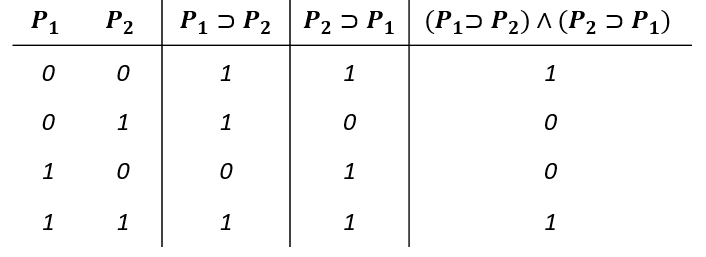
\includegraphics[width=0.5\linewidth]{4-4}
		\label{fig:4-4}
		\caption{Таблица к примеру 4.4}
	\end{figure}
	$(P_1 \lor \bar{P_2})\land (\bar{P_1}\lor P_2)$ - совершенная КНФ.\\
	Можно было бы воспользоваться $p\supset q\equiv \bar{p}\lor q \Rightarrow (P_1 \supset P_2)\land (P_2 \supset P_1)\equiv (\bar{P_1}\lor P_2)\land (\bar{P_2}\lor P_1)$.
\end{example}
Итак, далее будет считать, что нат дана формула $K=D_1 \land ... D_s$, где $D_1 \land ... D_s$ - дизъюнкты. Нам надо выяснить, выполнима $K=K(p_1 ,...,p_n)$ или нет.\\
Пусть $D_1 =(...\lor L \lor ...)$ и $D_2 =(... \lor \bar{L}\lor ...)$ два дизъюнкта: в первом есть литера $L$, во втором - $\bar{L}$(есть контрарная пара).
\begin{definition}
\textbf{Резольветой} $D_1$ и $D_2$ называется дизъюнкт $D$, получающийся из $D_1$ и $D_2$ вычеркиванием(удалением $L$ и $\bar{L}$) и объединением остальных членов $D_1$ и $D_2$.
\end{definition}
\begin{example}
	$D_1 =(L_1 \lor L_2 \lor L_3), D_2 =(L_1 , \bar{L}_2,\bar{L}_3), D=(\underbrace{L_1 \lor L_3}_{D_1 \setminus \{L_2\}}\lor \underbrace{L_1 \lor \bar{L}_3}_{D_2 \setminus \{\bar{L}\}})$.
\end{example}
Дизъюкт $D$(резольвента $D_1$ и $D_2$) будет обозначаться $\mathrm{Res}(D_1 ,D_2)$\\
$D_1 =S_1 \lor \cancel{L}, D_2 = S_2 \lor \cancel{\bar{L}}\Rightarrow D=S_1 \lor S_2,\quad\mathrm{Res}(D_1 ,D_2)=D$.\\
Если $D_1 =L$, а $D_2 =\bar{L}$(или наоборот), то $Res(L,\bar{L})=\emptyset$ - пустой дизъюнкт.\\
Обычно мы будем исследовать не формулы вида $(\Phi_1 \land ... \land \Phi_n \supset \Phi)\stackrel{?}{\equiv} 1$, а эквивалентную ей формулу $(\Phi_1 \land ... \land \Phi_n \land \bar{\Phi})\equiv 0$, то есть будет вести доказательство ``от противного''(то есть строить ``систему опровержения'').\\
\\
\textbf{(*)}Формула $\Phi$ выводима из $\{\Phi_1 ,...\Phi_n \}=S$ с помощью резолютивного вывода(метода), если существует такая последовательность формул $ \Phi_1^{'},...,\Phi_p^{'}$, что $\Phi_p^{'}=\Phi$, а любая $\Phi_1^{'},...,\Phi_p^{'}$ либо $\in S$, либо получена из $S$ по правилу (метод) резолюция.
\begin{theorem}
Если $S\supset \Phi$ по правилу (*), то $(S\supset \Phi)\equiv 1$.
\end{theorem}
\emph{Доказательство. } (От противного) $(S\supset \Phi)\equiv 1\Leftrightarrow (S\wedge\bar{\Phi})\equiv 0$ или $((\Phi_1\wedge\ldots\wedge\Phi_n)\wedge\bar{\Phi})\equiv 0$(**)\\
1. $\Phi\in S$, т.е. формула (**) имеет вид $(\Phi_1\wedge\ldots\wedge\underbrace{\Phi\wedge\Phi_i\ldots\Phi_n)\wedge}_{=0}\bar{\Phi}\Rightarrow$ (**) тоже $\equiv 0$.\\
2. $\Phi\in S$, доказываем методом математической индукции (по длине вывода - числу шагов в (*) равному $k$).\\
\underline{Базис индукции} $k=1$, т.е. $\Phi$ - получается из $S$ за один шаг (за одно применение правила резолюции) $\Rightarrow\exists \Phi_i=\Phi_i^{'}\vee L$ и $\Phi_j=\Phi_j^{'}\vee \bar{L}$ и $\Phi_i,\Phi_j\in S$ и $\mathrm{Res}(\Phi_i,\Phi_j)=\Phi$, т.е. $\mathrm{Res}(\Phi_i^{'}\vee L,\Phi_j^{'}\vee\bar{L})=c^{'}\vee c^{''}=\Phi$. Покажем, что если $\Phi_i,\Phi_j$ - тавталогии, то и $\Phi$ - тавталогия. Распишем это $(\Phi_i^{'}\vee L)\wedge(\Phi_j^{'}\vee\bar{L})\supset (\Phi_i^{'}\vee \Phi_i^{'}\vee\Phi_j^{'})$. Если $\Phi$ не тавтология, то найдется набор значений переменных, входящих в $\Phi$, на котором она обратится в $0$, т.е. $\Phi_i^{'}=0,\Phi_j^{'}=0$. Но $(\Phi_i^{'}\vee L)\wedge(\Phi_j^{'}\vee\bar{L})=1$ на этом же наборе $\underbrace{(\Phi_i\equiv 1,\Phi_j\equiv 1)}_{\text{по условию}}\Rightarrow (0\vee L)\wedge(0\vee\bar{L})=1$, т.е. $0=1$ - противоречие.\\
\underline{Предположение индукции} Пусть теорема верна для любого вывода длины (числа шагов) $=i<k$.\\
\underline{Индуктивный переход} (шаг индукции) Докажем теорему для $i=k$. Пусть имеется резолютивный вывод, $\Phi$ из $S=\{\Phi_1,\ldots,\Phi_n \}$ длины $k$, т.е.\\
$\Phi_1^{'},\Phi_2^{'},\ldots,\underbrace{\Phi_i^{'},\Phi_{i+1}^{'},\ldots,\Phi_j^{'}}_{\mathrm{Res}(\Phi_i^{'},\Phi_j^{'})=\Phi_k^{'}=\Phi},\ldots,\Phi_k^{'}=\Phi$. При этом $i,j<k$.\\
\underline{По предположению индукции} $(S\supset \Phi_i^{'})\equiv 1$, и $(S\supset \Phi_j^{'})\equiv 1\Rightarrow S\supset(\Phi_i^{'}\wedge \Phi_j^{'})\equiv 1$. Но $\Phi=\mathrm{Res}(\Phi_i^{'},\Phi_j^{'})$ и получена за один шаг $\Rightarrow(\Phi_i^{'}\wedge \Phi_j^{'})\supset \Phi$ тоже тавтология (см. базис индукции).\\
Итак, $S\supset \Phi_i^{'}\wedge \Phi_j^{'}$ - тавтология, $\Phi_i^{'}\wedge \Phi_j^{'}\supset\Phi$ тоже тавтология $\Rightarrow$ по свойству транзитивности $\Rightarrow(S\supset\Phi)\equiv 1$. Теорема доказана.\\
\\
Таким образом, метод резолюций не выводит нас из множества тавтологий. Заметим, что правило modus popens будет частным случаем: $D_1=L,D_2=D\vee \bar{L}\Rightarrow\mathrm{Res}(L,D\vee\bar{L})=D$.\\
Метод резолюций более удобен для компьютерной модели "доказательства от противного". Позже мы докажем главный результат этого раздела:
\begin{theorem}
Если множество дизъюнктов $D_1,\ldots D_n$ \underline{не выполнимо} то из него методом резолюций можно получить $\emptyset$ - дизъюнкт.
\end{theorem}
\section{Лекция 5}
%%%
%%%
	Покажем, что $\{P_1 \lor P_2 , P_1 \lor \bar{P_2}, \bar{P_1} \lor P_2 , \bar{P_1} \lor \bar{P_2}\}$ невыполнимо, то есть из него методом резолюции можно полусить $\emptyset$ - дизъюникт.\\
	$\underbrace{P_1\lor P_2}_{\circled{1}}, \underbrace{P_1\lor \bar{P_2}}_{\circled{2}},\underbrace{\bar{P_1}\lor P_2}_{\circled{3}},\underbrace{\bar{P_1}\lor \bar{P_2}}_{\circled{4}}$\\
	$\circled{1}+\circled{2} = P_1\lor P_1 \equiv \underbrace{P_1}_{\circled{5}}$ $\circled{5}+\circled{3} = \underbrace{P_2}_{\circled{6}}$ $\circled{6}+\circled{4} = \underbrace{\bar{P_1}}_{\circled{7}}$ $\circled{5}+\circled{7} = \emptyset$\\
	%\begin{figure}[!htbp]
	%	\centering
	%	\includegraphics[width=0.5\linewidth]{5-1}
	%	\label{fig:5-1}
	%\end{figure}
	Здесь мы изобразили получение(вывод) $\emptyset$ - дизъюникт в виде ``дерева''. На самом деле это списки дизъюнктов.\\
	$S=\{\underbrace{P_1\lor P_2}_{\circled{1}},\underbrace{P_1 \lor \bar{P_2}}_{\circled{2}},\underbrace{\bar{P_1}\lor P_2}_{\circled{3}},\underbrace{\bar{P_1}\lor \bar{P_2}}_{\circled{4}}\}\cup \{P_1,P_2,\bar{P_2},P_2\lor \bar{P_2}\}$.\\
	$\circled{1}+\circled{2} = P_1$ $\circled{1}+\circled{3} = P_2$	$\circled{2}+\circled{4} = \bar{P_2}$	$\circled{1}+\circled{4} = P_2\lor \bar{P_2}$
	%\begin{figure}[!htbp]
	%	\centering
	%	\includegraphics[width=0.5\linewidth]{5-2}
	%	\label{fig:5-2}
	%\end{figure}
	\begin{definition}
	Обозначим через $S_1 =[S]_{Res}^1$ множество дизъюнктов, которые можно получить из множества $S$ за одны шаг методом резолюций. $S_2 =[S]_{Res}^2 =[\{S\}\cup \{S_1\}]_{Res}^1 ,.., S_i =[S\cup \{S_1\}\cup ...\cup \{S_{i-1}\}]_{Res}^1$
	\end{definition}
	Любую литеру можно резольвировать столько раз, сколько требуется.
	Компюьтерная реализация(обсуждение).
	\begin{question}
		Как запрограммировать метод резолюций?
	\end{question}
		$S=\left\{\begin{array}{ll}
		(1) P\lor Q\\
		(2) \backsim P\lor Q\\
		(3) P\lor \backsim Q\\
		(4) \backsim P\lor \backsim Q \text{  получено из:}\\
		(5) Q \text{   из (1) и (2),}
		\end{array}\right.\\
		S_1=[S]_{Res}^1\left\{\begin{array}{ll}
		(6) P \text{   из (1) и (3),}\\
		(7) Q \lor \backsim Q \text{   из (1) и (3),}\\
		(8) P \lor \backsim P \text{   из (1) и (4),}\\
		(9) Q \lor \backsim Q \text{   из (2) и (3),}\\
		(10) P \lor \backsim P \text{   из (2) и (3),}\\
		(11) \backsim P \text{   из (2) и (4),}\\
		(12) \backsim Q \text{   из (3) и (4),}
		\end{array}\right.\\
		S_2 =[S]_{Res}^2\left\{\begin{array}{ll}
		(13) P \lor Q \text{   из (1) и (7),}\\
		(14) P \lor Q \text{   из (1) и (8),}\\
		(15) P \lor Q \text{   из (1) и (9),}\\
		(16) P \lor Q \text{   из (1) и (10),}\\
		(17) Q \text{   из (1) и (11),}\\
		(18) P \text{   из (1) и (12),}\\
		(19) Q \text{   из (2) и (6),}\\
		(20) \backsim P \lor Q \text{   из (2) и (7),}\\
		(21) \backsim P \lor Q \text{   из (2) и (8),}\\
		(22) \backsim P \lor Q \text{   из (2) и (9),}\\
		(23) \backsim P \lor Q \text{   из (2) и (10),}\\
		(24) \backsim P \text{   из (2) и (12),}\\
		(25) P \text{   из (3) и (5),}\\
		(26) P \lor \backsim Q \text{   из (3) и (7),}\\
		(27) P \lor \backsim Q \text{   из (3) и (8),}\\
		(28) P \lor \backsim Q \text{   из (3) и (9),}\\
		(29) P \lor \backsim Q \text{   из (3) и (10),}\\
		(30) \backsim Q \text{   из (3) и (11),}\\
		(31) \backsim P \text{   из (4) и (5),}\\
		(32) \backsim Q \text{   из (4) и (6),}\\
		(33) \backsim P \lor \backsim Q \text{   из (4) и (7),}\\
		(34) \backsim P \lor \backsim Q \text{   из (4) и (8),}\\
		(35) \backsim P \lor \backsim Q \text{   из (4) и (9),}\\
		(36) \backsim P \lor \backsim Q \text{   из (4) и (10),}\\
		(37) Q \text{   из (5) и (7),}\\
		(38) Q \text{   из (5) и (9),}\\
		(39) \emptyset \text{   из (5) и (12).}\\
 		\end{array}\right.\\$
 	(5)-(38) $Res$ 2 шага методом резольвент.\\
 	Появляется очень много резольвент.\\
 	\begin{Remark}
 		Пусть $D=(L_{i_1} \lor ... \lor L_{i_s})\equiv 1$, тогда множество дизъюнктов $S\equiv 1 \Leftrightarrow S \land D \equiv 1 (S\equiv 0 \Leftrightarrow S \land D \equiv 0)$. Иными словами дизъюнкт, являющийся тавтологией можно удалять из списка $[S]_{Res}^1.$
 	\end{Remark}
 		Для этого достаточно заметить, что если $\underbrace{D_1 \land ...\land D_n}_{S} \land D \underbrace{\equiv}_{D\equiv 1} D_1 \land ... \land \underbrace{D_n \land 1}_{D_n}=\underbrace{D_1 \land ... \land D_n}_{S}$.
 	\begin{proposition}
 		Дизъюнкт $D \equiv 1 \Leftrightarrow$ в нем есть хотя бы одна контрараная пара литер.
 	\end{proposition}
 	\underline{Доказательство}\\
 	$\Rightarrow$\\
 	Пусть в $D$ есть контрарная пара литер $L_i$ и $\bar{L_i};D=(...\lor L_i \lor ... \lor \bar{L_i} \lor ...)\underbrace{=}_{\text{коммутативн.}``\lor''}(...\lor L_i \lor \bar{L_i} \lor ...)=(... \lor 1 \lor ...) \equiv 1$.\\
	$L_i \lor \bar{L_i} \equiv 1 \Rightarrow$ если $L_i=P_{j_i}$ то $\bar{L_i}=\bar{P_{j_i}} \Rightarrow L_i \lor \bar{L_i} = P_{j_i}\lor \bar{P_{j_i}}\equiv 1$.\\
	Аналогично если $L_i = \bar{P_{j_i}}$ то $\bar{L_i}=\bar{\bar{P_{j_i}}}=P_{i_j}\Rightarrow P_{i_j}\lor \bar{P_{i_j}} \equiv 1$.\\
	$\Leftarrow$\\
	Пусть в $D$ нет контрарной пары, а $D\equiv 1$. Если нет контрарной пары, то $D$ имеет вид: $D=(P_{i_1}^{\sigma_{i_1}},...,P_{i_n}^{\sigma_{i_n}})$ и все $P_{i_j} (j=1\ldots n)$ разные. Утверждение доказано.\\
	\\
	С учетом утверждения 1 тожно уменьшить число резольвент, соблюдая правила:\\
	(1)	$D\lor D \equiv D$ (удаление дублей)\\
	(2) $D\equiv 1$ (удаление тавтологий)\\
	Постмотрим как сократится вывод (со стр. 2)\\
	$\left.\begin{array}{ll}
		(1) P\lor Q\\
		(2) \backsim P\lor Q\\
		(3) P\lor \backsim Q\\
		(4) \backsim P\lor \backsim Q \text{  получено из:}\\
	\end{array}\right\}\\
		(5) Q \text{   из (1) и (2),}\\
		(6) P \text{   из (1) и (3),}\\
	\left.\begin{array}{ll}
		\cancel{(7) Q \lor \backsim Q} \text{   из (1) и (3),}\\
		\cancel{(8) P \lor \backsim P} \text{   из (1) и (4),}\\
		\cancel{(9) Q \lor \backsim Q} \text{   из (2) и (3),}\\
		\cancel{(10) P \lor \backsim P} \text{   из (2) и (3),}\\
	\end{array}\right\}\text{тавталогии}\\
		(11) \backsim P \text{   из (2) и (4),}\\
		(12) \backsim Q \text{   из (3) и (4),}\\
		(13) P \lor Q \text{   из (1) и (7),}\\
	\left.\begin{array}{ll}
		\cancel{(14) P \lor Q} \text{   из (1) и (8),}\\
		\cancel{(15) P \lor Q} \text{   из (1) и (9),}\\
		\cancel{(16) P \lor Q} \text{   из (1) и (10),}\\
		\cancel{(17) Q} \text{   из (1) и (11),}\\
		\cancel{(18) P} \text{   из (1) и (12),}\\
		\cancel{(19) Q} \text{   из (2) и (6),}\\
	\end{array}\right\}\text{дубли}\\
		(20) \backsim P \lor Q \text{   из (2) и (7),}\\
	\left.\begin{array}{ll}
		\cancel{(21) \backsim P \lor Q} \text{   из (2) и (8),}\\
		\cancel{(22) \backsim P \lor Q} \text{   из (2) и (9),}\\
		\cancel{(23) \backsim P \lor Q} \text{   из (2) и (10),}\\
		\cancel{(24) \backsim P} \text{   из (2) и (12),}\\
		\cancel{(25) P} \text{   из (3) и (5),}\\
		\cancel{(26) P \lor \backsim Q} \text{   из (3) и (7),}\\
		\cancel{(27) P \lor \backsim Q} \text{   из (3) и (8),}\\
		\cancel{(28) P \lor \backsim Q} \text{   из (3) и (9),}\\
		\cancel{(29) P \lor \backsim Q} \text{   из (3) и (10),}\\
		\cancel{(30) \backsim Q} \text{   из (3) и (11),}\\
		\cancel{(31) \backsim P} \text{   из (4) и (5),}\\
		\cancel{(32) \backsim Q} \text{   из (4) и (6),}\\
		\cancel{(33) \backsim P} \lor \backsim Q \text{   из (4) и (7),}\\
		\cancel{(34) \backsim P} \lor \backsim Q \text{   из (4) и (8),}\\
		\cancel{(35) \backsim P} \lor \backsim Q \text{   из (4) и (9),}\\
		\cancel{(36) \backsim P} \lor \backsim Q \text{   из (4) и (10),}\\
		\cancel{(37) Q} \text{   из (5) и (7),}\\
		\cancel{(38) Q} \text{   из (5) и (9),}\\
	\end{array}\right\}\text{дубли}\\
		(39) \emptyset \text{   из (5) и (12).}\\
	$
	введем \underline{третье правило} (упорядочение букв в дизъюнктах) например:\\
	$\underbrace{P_1}_{\text{старшая буква}}\geqslant P_2\geqslant P_3$ Начинаем делать операцию с начала по старшей букве $P_1$, потом $P_2$, потом $P_3$.\\
    $S=\{\underbrace{P_1\lor P_2}_{\circled{1}},\underbrace{P_1 \lor \bar{P_2}}_{\circled{2}},\underbrace{\bar{P_1}\lor P_2}_{\circled{3}},\underbrace{\bar{P_1}\lor \bar{P_2}}_{\circled{4}}\}$\\
	$\circled{1}+\circled{3} = P_2$\\
	$\circled{1}+\circled{4} = \bar{P_2}$\\
	$\circled{2}+\circled{3} = \cancel{(P_2 \lor \bar{P_2})\equiv 1}$  - тавтология больше.\\
	$\circled{2}+\circled{4} = \cancel{\bar{P_2}\text{ - дубль}}$  - тавтология больше.\\	
	%\begin{figure}[!htbp]
	%	\centering
	%	\includegraphics[width=0.5\linewidth]{5-3}
	%	\label{fig:5-3}
	%\end{figure}
	$S_1 =S\cup \{P_2,\bar{P_2}\}$ - по $P_1$ больше нет резольвент, начинаем с $P_2$.\\
	$S_1=\{\underbrace{P_1\lor P_2}_{\circled{1}},\underbrace{P_1 \lor \bar{P_2}}_{\circled{2}},\underbrace{\bar{P_1}\lor P_2}_{\circled{3}},\underbrace{\bar{P_1}\lor \bar{P_2}}_{\circled{4}},\underbrace{P_2}_{\circled{5}},\underbrace{\bar{P_2}}_{\circled{6}}\}$\\
	$\circled{1}+\circled{2} = P_1$\\
	$\circled{1}+\circled{4} = \cancel{P_1 \lor \bar{P_1}}$ - тавтологии.\\
	$\circled{2}+\circled{3} = \cancel{\bar{P_1} \lor \bar{P_1}}$ - тавтологии.\\
	$\circled{3}+\circled{4} = \bar{P_1}$\\
	$\circled{5}+\circled{6} = \emptyset$\\
	%\begin{figure}[!htbp]
	%	\centering
	%	\includegraphics[width=0.5\linewidth]{5-4}
	%	\label{fig:5-4}
	%\end{figure}
	Четвертое правило(предпочтение однолитеральным дизъюнктам).\\
	Резольвируем сначала однолитерные дизъюнкты(если они есть).\\
%%%
%%%
%%%
$S_1=\{P_1\vee P_2,P_1\vee \bar{P}_2,\bar{P}_1\vee P_2,\bar{P}_1\vee\bar{P}_2, P_2,\bar{P}_2\}$, где $P_2,\bar{P}_2$ - однолитерные дизъюнкты $\Rightarrow \emptyset$.\\
\textbf{Использование интерпретации}.\\
Пусть $S=\{D_1,\ldots,D_n \}$ не выполнимое множество дизъюнктов, т.е. $D_1\wedge\ldots\wedge D_n\equiv 0$ зависящее от переменных $P_1,\ldots,P_n$. $I_n$ - некоторая интерпретация этого множества $S$, то $I_n=\{P_1=\alpha_1^{\sigma_1},\ldots,P_n=\alpha_n^{\sigma_n} \}$, где $\alpha_i^{\sigma_i}=\{0,1\}$.\\
Напомню обозначение из курса дискретной математики: $P^{\sigma}=(P\wedge\sigma)\vee(\bar{P}\wedge\bar{\sigma})$, $P$ - булевская переменная, $\sigma$ - константа $\{0,1 \}$. Например: $P^0=(P\wedge 0)\vee (\bar{P}\wedge \bar{0})=\bar{P},P^1=(P\wedge 1)\vee (\bar{P}\wedge \bar{1})=P$. \\
При фиксированной интерпретации $I_n$ множество $S=S_{I_n}^0\bigcup S_{I_n}^1$, где $S_{I_n}^0$ - множество тех дизъюнктов $S$, которые $=0$ при этой интерпретации, а $S_{I_n}^1$ - которые равны $1$.
\begin{proposition}
	Для любого невыполнимого множества дизъюнктов $S$ имеем $S_{I_n}^0\ne \emptyset$ и $S_{I_n}^1\ne \emptyset$ при любой интерпретации $I_n$.
\end{proposition}
\emph{Доказательство.} Если $S_{I_n}^0=\emptyset\Rightarrow$ на $I_n$ все дизъюнкты из $S$ принимают значения $1$, т.е. множество $S$ - выполнимо $\Rightarrow$ противоречие. Если $S_{I_n}^1=\emptyset\Rightarrow$ в дизъюнктах из $S$ нет ни одной \underline{контрарной пары} литер, т.е. присутствуют $L=P_i^{\sigma_i}$, но нет $\bar{L}=P_i^{\bar{\sigma}_i}$, присвоим $P_i=\sigma_i\Rightarrow$(см. напоминание стр. 6)$\Rightarrow$ все дизъюнкты из $S$ будут на этой интерпретации $I_n(I_n=\{P_1=\sigma_1,\ldots,P_n=\sigma_n \})$ будут равны $1$. То есть, множество $S$ будем выполнимым. Противоречие.
\begin{example}
	$S=\{(P_1\vee P_2\vee \bar{P}_3),(P_1\vee \bar{P}_3) \},I_1=\{P_1=1,P_2=1,P_3=0 \},(1\vee 1\vee \bar{0}=1),(1\vee \bar{0})=1\Rightarrow S=1$ на $I_1$. 
\end{example}
Используем интерпретацию следующим образом: Фикструем $I_n$, представляем $S=S_{I_n}^0\bigcup S_{I_n}^1$. $S_{I_n}^0,S_{I_n}^1$ - $\mathrm{Res}$, т.е. внутри $S_{I_n}^0$ и внутри $S_{I_n}^1$ дизъюнкты не резольвируются. $\mathrm{Res}$ ищется только между дизъюнктами из $S_{I_n}^0$ и $S_{I_n}^1$.
\begin{example}
	$S=\{ P_1\vee P_2,P_1\vee P_3,P_1\vee \bar{P}_2\vee\bar{P}_3,\bar{P}_1 \},I_n=(0,0,0),S_{(0,0,0)}^0=\{P_1\vee P_2,P_1\vee P_3 \},S_{(0,0,0)}^1=\{P_1\vee \bar{P}_2\vee \bar{P}_3,\bar{P}_1 \}$ \\
	Из них: $P_1\vee\bar{P_3},P_2,P_1\vee \bar{P}_2,P_3$. $\big[ S^0_{(0,0,0)}\big]^1=S^0_{(0,0,0)}\bigcup \{P_2,P_3 \},\big[ S^1_{(0,0,0)}\big]^1=S^1_{(0,0,0)}\bigcup \{P_1\vee \bar{P}_3,P_1\vee \bar{P}_2 \}$.\\
	$\{P_1\vee P_2,P_1\vee P_3,P_2,P_3\},\{ P_1\vee \bar{P}_2\vee \bar{P}_3,\bar{P}_1 ,P_1\vee \bar{P}_3,P_1\vee \bar{P}_2\}$.\\
	Из них: $P_1$(4-ая с 3-ой), потом $P_1$ с $\bar{P}_1$ получаем $\emptyset$.
\end{example}
Выбранная интерпретация в процессе вывода $\emptyset$ - дизъюнкта не меняется.\\
Частая ошибка студентов при реализации задач: $S=\{p\vee q,\bar{p}\vee\bar{q} \}\Rightarrow \emptyset$ - это не верно.\\
Надо попарно получить $(q\vee \bar{q}),(p\vee\bar{p})$ - тавтологии, а не $\emptyset$ - дизъюнкт.
\section{Лекция 6}
Пусть $S=\{D_1,\ldots,D_n \}$ - некоторое множество дизъюнктов. 
\begin{definition}
Обозначим через $|S|$ \textbf{число дизъюнктов} в $S$, а через $\|S\|$ - \textbf{число вхождений литер} во все дизъюнкты из $S$. Каждая литера считается столько раз, сколько она входит в дизъюнкты из $S$.
\end{definition}
\begin{example}
	$S=\{p,p\vee q,\bar{p}\vee \bar{q}\vee r \},|S|=3,\|S\|=1+2+3=6$.
\end{example}
\begin{proposition}
	$\|S\|\geqslant |S|$.
\end{proposition}
Введем величину $k(S)=\|S\|-|S|,k(S)\geqslant 0$.
\begin{theorem}
(Анрерсен) о полноте метода резолюций для исчисления высказываний.\\
Пусть $S$ - невыполнимое множество дизъюнктов. Тогда методом резолюций (резолютивним выводом) из $S$ можно получить $\emptyset$-дизъюнкт.
\end{theorem}
\underline{\emph{Доказательство}} Индукция по $k(S)=\|S\|-|S|$.\\
\underline{Базис индукции} $k(S)=0\Leftrightarrow$\\
1) Все дизъюнкты в $S$ однолитерные, т.е. $S=\{L_{i_1},\ldots,L_{i_n} \}$.\\
2) $S=\{L_{i_1}\vee L_{i_j},L_{i_2},\ldots,L_{i_n},\emptyset \}$.\\
Рассмотрим 1). В этом случае в $S$ есть контрарная пара $L_i=L,L_j=\bar{L}$ (иначе $S$ выполнимо) $\Rightarrow\mathrm{Res}(L_i,L_j)=\mathrm{Res}(L,\bar{L})=\emptyset$. \\
2) $S=\{L_{i_1}\vee L_{i_2},L_{i_3},\ldots,L_{i_{n-1}},L_n=\emptyset \},k(S)=0$. В этом случае $\emptyset$-дизъюнкт $\in S$ и получается за $0$-шагов метода резолюций. $\emptyset$-дизъюнкт просто логическое следствие из множества формы $S$.\\
\underline{Предположение индукции} Пусть теорема верна для всех $S$, у которых $k(S)<n$.\\
\underline{Индуктивный переход} Докажем теорему для всех $S:k(S)=n$. Если $\emptyset$-дизъюнкт $\in S$, то очевидно, что теорема верна. Можно рассматривать такие $S$, что $\emptyset$-дизъюнкт $\notin S$. Так как $k(S)>0$, то в $S$ существует хотя бы один дизъюнкт вида $D=(D^{'}\vee L)$, где $L$ - литера, и $D^{'}\ne \emptyset$-дизъюнкт. Рассмотрим множество $S^{'}=S\setminus \{D^{'}\vee L \}$ и образуем два множества дизъюнктов $S_1=S^{'}\bigcup\{D^{'}\},S_2=S^{'}\bigcup{L}$. Очевидно, что $|S_1|=|S_2|=|S|$ - число дизъюнктов в $S_1$ и $S_2$ такое же, как в $S$, но $k(S_2)\leqslant k(S_1)<k(S)$, т.к. в $S_1$ на одну литеру меньше, а в $S_2$, по-крайней мере на одну литеру меньше. $\|S_1\|=\|S\|-1,\|S_2\|=\|S\|=\|D^{'}\|$, и $\|D^{'}\|\geqslant 1$.\\
Докажем теперь, что $S_1$ и  $S_2$ невыполнимые множества, если невыполнимо $S$(оно не выполнимо по условию теоремы).\\
Пусть $I$-множество всех интерпретаций $S$. (Это множество всех двоичных наборов $2^n$, где $n$-число \underline{различных переменных} в дизъюнктах из $S$). $S\equiv 0$ на $I$ по условию теоремы.\\
\begin{figure}[!htbp]
	\centering
	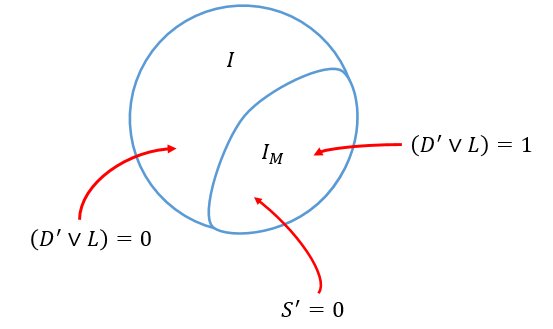
\includegraphics[width=0.5\linewidth]{6-1}
	\label{fig:6-1}
	\caption{К доказательству теоремы 6.1}
\end{figure}
$I_m\subset I$ - множество интерпраций на которых выполнима формула $D^{'} \lor L$. $I_M\ne \emptyset$ - очевидно. На $I_M$ множество формул $S^{'}$ не выполнимо(иначе бы было выполнимо $S$).\\
Следовательно и $S_1 = D^{'} \cup S^{'},S_2=L\cup S^{'}$ тоже не выполнимы на $I_M$.\\
На множестве $I\backslash I_M$ формула $(D^{'} \lor L)=0 \Rightarrow D^{'} =0, L=0 \Rightarrow S_1 = S^{'} \cup D^{'}$ и $S_2 =L\cup D^{'}$ тоже не выполнимы на $I\backslash I_M$. Следовательно и $S_1$ и $S_2$ не выполнимы на $I$.\\
Отсюда(т.к. $K(S_1)<n, K(S_2)<n$ и оба они невыполнмы) по предположению индукциии из $S_1$ за $i$ шагов можно получить $\phi$-дизъюнкт, а из $S_2$ за $j$ шагов тоже можно получить $\phi$-дизъюнкт.\\
Рассмотрим два случая:\\
а) при выводе $\phi$-дизъюнкта из $S_1 = S^{'}\cup D^{'}$ дизъюнкт $D^{'}$ не использовался. Тогда этот вывод одновременно есть и вывод $\phi$-дизъюнкта из $S$.\\
б) дизъюнкт $D^{'}$ использовался. В этом случае вместо $D^{'}$ поставим исходный дизъюнкт $(D^{'}\lor L)=D$, тогда в этом выводе $\phi$-дизъюнка мы получим или $\phi$-дизъюнкт или дизъюнкт $L$.\\
$D^{'} \longrightarrow D^{''} \longrightarrow ... \longrightarrow D^{(i)}=\emptyset$.\\
$D^{'}\lor L \longrightarrow D^{''}\lor L\longrightarrow ... \longrightarrow D^{(i)}\lor L = \emptyset \lor L = L$.\\
Но по предположению индукуии из $S_2 =S^{'}\cup L$ за $j$ шагов можно получить $\phi$-дизъюнкт. Тогда из $S$ за $\sigma \le i+j$ тоже можно получить $\phi$-дизъюнкт. Теорема даказана.\\
\\
\underline{Напомню}, что $S=S^{'}\cup \{D^{'}\lor L\},S_1 = S^{'}\cup \{D^{'}\},S_2 =S^{'}\cup \{L\}$.\\
Заметим, что если из $S \supset \emptyset$, то $S$ не выполнимо. Для этого контрарную пару $3L, \bar{L}$ заменим на эквивалентные им формулы $L\lor 0, \bar{L}\lor 0\Rightarrow Res(L\lor 0,\bar{L}\lor 0)=0$(ложь), то есть 0 логическое следствие $S\Rightarrow (S\supset 0)\equiv 1$ то есть $S$ не выполнимо.\\
Можно выяснение истинности или ложности высказываний свести к решению систем алгебраических уравнений.\\
``Истина'' - $1\quad\bar{p}\quad p\wedge q\quad p\vee q$.\\
``Ложь'' - $0\quad 1-p\quad p\cdot q\quad p+q-p\cdot q$.\\
$\Rightarrow p\supset q = \bar{p}\vee q=(1-p)+q-(1-p)q=1-p+p\cdot q$.\\
Но!!! Степень нелинейности возрастает $p\vee q\vee r=p+q-p\cdot q+r-(p+q-pq)r$.\\
Докажем, например, что $p\supset r$ является логическим следствием формул $(p\supset q)$ и $(q\supset r)$, т.е. если $(p\supset q)\wedge(q\supset r)=1$, то и $(p\supset r)=1$. Переписываем это в виде алгебраических уравнений. \\
$(p\supset q)=1\Rightarrow 1-p+p\cdot q=1,(q\supset r)=1\Rightarrow 1-q+q\cdot r=1$. Надо показать, что $1-p+p\cdot r=1$, если
\begin{equation*}
\left\{\begin{array}{l}
1-p+p\cdot q=1\Leftrightarrow p(1-q)=0\quad (1)\\
1-q+q\cdot r=1\Leftrightarrow q(1-r)=0\quad (2)
\end{array}\right.
\end{equation*}
Варианты:\\
1.1) $p=0,q=0\to r=0\text{ или } r=1$.\\
1.2) $p=0,q=1\to r=1$.\\
2) $p=1,q=1 \,(1)\to \text{ из }(2) r=0$.\\
Итак, при $p=0,1-p+pr=1$,\\
при $p=1$ из (1) $\Rightarrow q=1$, из (2) $\Rightarrow r=1\Rightarrow$,\\
Надо проверить наборы
\begin{equation*}
\begin{aligned}
&\quad p\quad q\quad r\\
&\left.\begin{array}{l}
0\quad 0\quad 0\\
0\quad 0\quad 1\\
0\quad 1\quad 1\\
\end{array}\right\} 1-p+pr=1\Leftrightarrow 1=1, \text{ т.к. } p=0.\\
&\quad 1\quad 1 \quad 1 \quad 1-1+1\cdot 1=1,\text{ т.е. } (p\supset r) - \text{ логическое следствие } 
\end{aligned}
\end{equation*}
\begin{example}
\underline{Пример-задача}\\
База данных(БД)=$\{\alpha_1,\alpha_2,\alpha_3,\alpha_4\}$.\\
База знаний(БЗ)=$\{(\alpha_1 \land \alpha_2)\supset (\alpha_5 \land \alpha_6),(\alpha_4 \land \alpha_3)\supset(\alpha_7),(\alpha_7 \land \alpha_6)\supset \alpha_8\}$.\\
БД - это факты из ПО (аксиомы ПО).\\
БД - это знания(что делать) о фактах ПО.\\
Система извлечения знаний: БД$\cup$БЗ.\\
\underline{Вопрос к системе:} можно ли получить $\alpha_8$?
\end{example}
Сводим вопрос к логическому следствию\\
$(((\alpha_1 \land \alpha_2)\supset (\alpha_5 \land \alpha_6))\land ((\alpha_4 \land \alpha_3)\supset \alpha_7)\land ((\alpha_7 \land \alpha_6)\supset \alpha_8))\land \alpha_1 \land \alpha_2 \land \alpha_3 \land \alpha_4) \supset \alpha_8$, то есть является ли $\alpha_8$ логическим следствием формул из БД$\cup$БЗ?\\
Преобразуем формулы к дизъюнктам $((\bar{\alpha_1}\lor \bar{\alpha_2}\lor \alpha_5)\land (\bar{\alpha_1}\lor \bar{\alpha_2}\lor \alpha_6)\land (\bar{\alpha_3}\lor \bar{\alpha_4}\lor \alpha_7)\land (\bar{\alpha_4}\lor \bar{\alpha_3}\lor \alpha_7)\land \alpha_1 \land \alpha_2 \land \alpha_3 \land \alpha_4 \land \bar{\alpha_8})\equiv 0$ то есть надо доказать невыполнимость этой формулы.\\
$\underbrace{\bar{\alpha_1}\lor \bar{\alpha_2}\lor \alpha_5}_{\text{этот дизъюнкт не потребовался}},\underbrace{\bar{\alpha_1}\lor \bar{\alpha_2}\lor  \alpha_6}_{\circled{1}},\underbrace{\bar{\alpha_4}\lor \bar{\alpha_3}\lor \alpha_7}_{\circled{2}},\underbrace{\bar{\alpha_7}\lor \bar{\alpha_6}\lor \alpha_8}_{\circled{3}},\underbrace{\alpha_1}_{\circled{4}},\underbrace{\alpha_2}_{\circled{5}},\underbrace{\alpha_3}_{\circled{6}},\underbrace{\alpha_4}_{\circled{7}},\underbrace{\bar{\alpha_8}}_{\circled{8}}$\\
$\circled{1}+\circled{5}=\underbrace{\bar{\alpha_1}\lor \alpha_6}_{\circled{9}};\circled{2}+\circled{6}=\underbrace{\bar{\alpha_4}\lor \alpha_7}_{\circled{10}};$ $\circled{9}+\circled{4}=\underbrace{\alpha_6}_{\circled{11}};\circled{10}+\circled{7}=\underbrace{\alpha_7}_{\circled{12}};$\\
$\circled{11}+\circled{3}=\underbrace{\bar{\alpha_7}\lor \alpha_8}_{\circled{13}}$; $\circled{13}+\circled{12}=\underbrace{\alpha_8}_{\circled{14}}$; $\circled{14}+\circled{8}=\emptyset$\\
\underline{Ответ:} Да, $\alpha_8$ можно получить.\\
Переменные $\alpha_1 \ldots \alpha_8$ могут быть любой природы - это могут быть химические формулы, технологические процессы и т.д.
\begin{Remark}
	Пусть $S_1$ - невыполнимое множество формул, а $S_2$ - любое множество формул. Тогда множество $S=S_1 \cup S_2$ тоже невыполнимо.\\
\end{Remark}

\section{Лекция 7}
Метод резолюции и его вариант с использованием интерпретации невыполнимого множества $S$ обладают свойством полноты, т.е. $\emptyset$-дизъюнкт $\in[S]_{\mathrm{Res}}$. В большинстве задач невыполнимое множество формул $S$ можно представить в виде $S=A\cup \Phi$, где $A=\{A_i \}$ - аксиомы предметной области, а $\Phi=\{\Phi_j \}$ - множество всех формул, которые мы хотим доказать, т.е. $\forall \Phi_j\in\Phi\Rightarrow (A\wedge \bar{\Phi}_i)\equiv 0$.\\
$\overbrace{\underbrace{A_1,\ldots,A_n}_{A}\quad \underbrace{\bar{\Phi}_1,\ldots,\bar{\Phi}_m}_{\bar{\Phi}}}^{S}$.\\
Если $A$ - это множество аксиом ПО, то оно должно быть непротиворечивым и при невыполнимом $S$ $\emptyset$-дизъюнкт может быть получен $\mathrm{Res}(B_1,B_2)$, где один из дизъюнктов $B_1$ и $B_2$ принадлежит $\bar{\Phi}$. Т.е. получение резольвент выглядит так:\\
$A\quad \underbrace{\Phi\cup\{\text{ все резольвенты из } S \text{ вида } \mathrm{Res}(B_1,B_2)}_{\text{несущее множество } T}\}$.\\
Из них образуется $\mathrm{Res}(B_1^{'},B_2^{'});$ если $B_1^{'}\in A$, то $B_2^{'}\in T$ и наоборот. Внутри $A$ $\mathrm{Res}$ запрещено по определению.\\
Зачем эта процедура нужна? Цель - уменьшит число резольвент. Как правило $|A|>>|\Phi|$. 
\begin{definition}
	Пусть $S$ - невыполнимое множество назовем $S_H\subseteq S$ \textbf{наименьшим невыпольнимым множеством}, если:\\
	1) $S_H$ - невыполнимо\\
	2) $\forall S^*\subset S_H$, множество $S^*$ - выполнимо.
\end{definition}
Заметим, что если $S_H\subseteq S$ наименьшее невыполнимое множество, то $\emptyset$-дизъюнкт можно искать так: $\forall c\in S_H$ $\underbrace{S_H\setminus \{c\}}_{\text{множество }A}\quad \underbrace{\{\bar{c}\}\cup\{\text{все резольвенты }\mathrm{Res}(B_1,B_2)\}}_{\text{несущее множество }T}$.\\
Из них получить $\mathrm{Res}$. $S_H\setminus \{c\}$ - выполнимо по определению $S_H$, т.е. это аналог аксиом ПО. Искать $S_H$ - трудно.
\begin{example}
(Самостоятельно)\\
$S=\{p\vee q,\bar{p}\vee \bar{r},p\vee q\vee r,\bar{p}\vee\bar{q},\bar{q}\vee\bar{r},p,q,r \}$ Найти $S_H$, если их несколько, найти все $S_H\supseteq S$.\\
\\
\textbf{Линейная резолюция}
\end{example}
\begin{definition}
	Для заданного множества дизъюнктов $S$ и дизъюнктов $C_0\in S$ \textbf{линейный вывод (линейная резолюция)} дизъюнкта $S_n\in S$ c верхним дизъюнктов $C_0$ - это вывод, имеющий следующий вид: (см. рис 7.1). При этом\\
	1. $\forall i=0,1,\ldots,n-1$ дизъюнкт $C_{i+1}=\mathrm{Res}(C_i,B_i)$.\\
	2. $\forall B_i$ либо $\in S$, либо есть $C_j$ для $i<j$.\\
\end{definition}
\begin{figure}[!htbp]
    \centering
	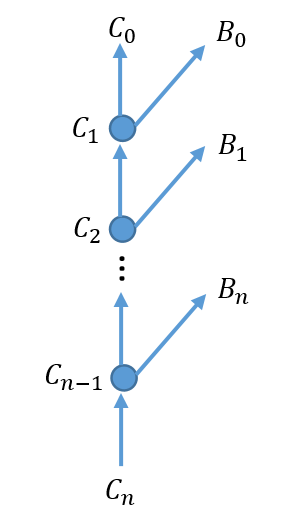
\includegraphics[width=0.2\linewidth]{7-1}
	\label{fig:7-1}
	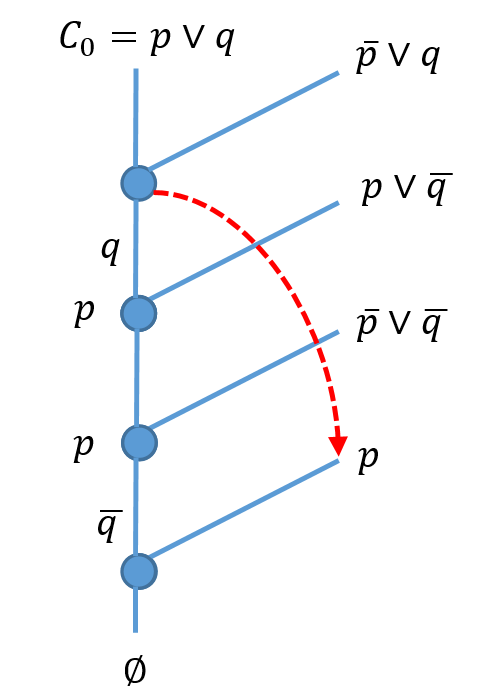
\includegraphics[width=0.2\linewidth]{7-2}
	\label{fig:7-2}
	\caption{Линейная резолюция / К примеру 7.2}
\end{figure}
\begin{definition}
	$C_i$ называется \textbf{центральным дизъюнтком}. $B_i$ называется \textbf{боковым дизъюнтком}. 
\end{definition}
\begin{example}
	$S=\{p\vee q,\bar{p}\vee q,p\vee \bar{q},\bar{p}\vee\bar{q}\}$
\end{example}
Можно доказать следующее 
\begin{proposition}
	Если $S_H\in S$ - наименьшее невыполнимое множество дизъюнктов, то существует линейный вывод $\emptyset$-дизъюнкт с верхним дизъюнтком $C\in S_H$.
\end{proposition}
\underline{Важно} Утверждение не гарантирует, что $\forall C\in S_H$ можно получить $\emptyset$-дизъюнкт. Пусть $S_H=\{C_1,\ldots,C_n \}$
\begin{figure}[!htbp]
	\centering
	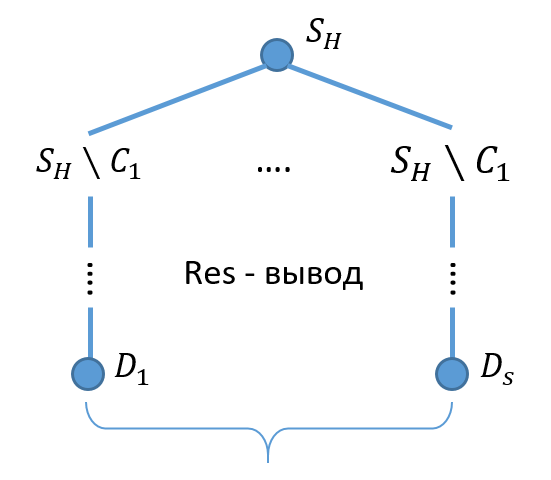
\includegraphics[width=0.3\linewidth]{7-3}
	\label{fig:7-3}
	\caption{Важно отметить!}
\end{figure}
Выводы $\emptyset$-дизъюнкта могут быть разной длины. \\
$\emptyset$ есть среди $\{D_1,\ldots,D_s \}$, но какие $D_i=\emptyset$-дизъюнкт мы не знаем.(перебор!) Все стратегии получения $\emptyset$-дизъюнкта, которые мы рассматривали до этого обладали свойством полноты, т.е. гарантировали получение $\emptyset$-дизъюнкта из $S$ при выпольнимости его.\\
\textbf{Эвристики} - стратегии не обладающие свойством полноты, но в \underline{отдельных случаях} позволяющие быстро получить результат. Например, те, которые мы уже раньше сформултровали:\\
1) Удаление дублей: $D\vee D=D$.\\
2) Удаление тавтологий $D\equiv 1$.\\
3) Упорядочение букв в дизъюнктах $P_1\geqslant P_2\geqslant \ldots\geqslant P_n$ и резольвирование букв по старшинству.\\
Можно добавить еще одино правило:\\
4) Если в $S$ есть $D=D_1D_2$ и есть $D_1$, то $D$ можно удалить $S$. Это не влияет на невыполнимость: $D_1\vee D_1D_2=D_1(1\vee D_2)=D_1$.\\
\\
Правило формулируется так: ``короткий'' дизъюнкт поглощает ``длинный'' дизъюнкт.\\
Ещё можно предложить такую стратегию. Вывод выглядит так: $S=\{S_1,\ldots,S_n \}\cup\{S_0\}$, где $\{S_0\}$ - выделенный дизъюнкт.
\begin{figure}[!htbp]
	\centering
	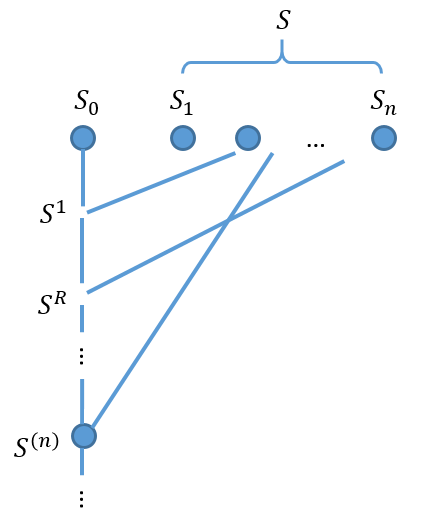
\includegraphics[width=0.3\linewidth]{7-4}
	\label{fig:7-4}
	\caption{S-резолюция}
\end{figure}
Все боковые дизъюнкты из $S$ и верхний дизъюнкт $S_0$.\\
Это частный случай линейной резолюции. В линейной резолюции разрешается использовать $S^{(1)},\ldots,S^{(n)}$. Назовем этот процесс \textbf{$S-$резолюцией (или входной резолюцией)}.\\
\\
\textbf{E-резолюция(единичная резолюция)}
\begin{definition}
	В \textbf{$E$-резолюции} по-крайней мере один из дизъюнктов - литерал (единичный дизъюнкт), т.е. $\forall$ шаг вывода есть $\mathrm{Res}(A_i,A_j)$, где $A_i$ или $A_j$ (или оба вместе) есть $L$ или $\bar{L}$.
\end{definition}
\begin{definition}
	\textbf{S-опровержение и Е-опровержение} - это вывод из $S$ $\emptyset$-дизъюнкта $E-$(соответственно $S-$) резолюцией. Эти процедуры не обладают свойством полноты.
\end{definition}
\begin{theorem}
	Для невыполнимого множества дизъюнктов $S$ существует $E$-опровержение $\Leftrightarrow$ существует $S-$опровержение.
\end{theorem}
\textbf{Использование оценочных функций}
\begin{figure}[!htbp]
	\centering
	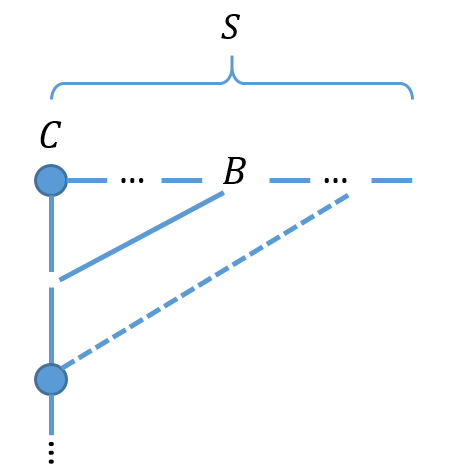
\includegraphics[width=0.3\linewidth]{7-5}
	\label{fig:7-5}
	\caption{Использование оценочных функций}
\end{figure}
Пусть есть резолютивный вывод \underline{начинающийся} с верхнего дизъюнкта $C$ и бокового дизъюнкта $B$, где $C,B\in$ некоторому множеству дизъюнктов $S$. Обозначим через $L^*(C,B)$ \textbf{наименьшее число шагов} метода $\mathrm{Res}$ для получения $\emptyset$-дизъюнкта из этой пары $(C,B)$. Обычно можно построить некоторые примеры для некоторых пар $(C_1,B_1),\ldots,(C_n,B_n) \to L^*(C_1,B_1),\ldots,L^*(C_n,B_n)$ - примеры просто подсчитаны (например в ручную).\\
\\
Введем ещё понятие \textbf{характеристической функции} пары $(C,B)$\\
1) $f_1(C,B)=$ число литер в $C$ (или в $B$).\\
2) $f_2(C,B)=$ число боковых дизъюнктов, которые можно резольвировать с $C$.\\
3) $f_3(C,B)=$ длина $C$ + длина $B$ - 2.\\
\ldots\\
Эти функции легко вычислить. Можно придумать много таких полезных характеристических функций пар. Рассмотрим функцию пар следующего вида:
\begin{equation*}
L(C,B)=W_0+W_1\cdot f_1(C,B)+\ldots+W_n\cdot f_n(C,B).
\end{equation*}
где $f_1,\ldots,f_n$ - характеристические функции пар.\\
\\
\underline{Гипотеза:} Функцию $L^*$ можно ``хорошо'' аппроксимировать линейной комбинацией характеристических функций $f_1,\ldots,f_n$, например, методом наименьших квадратов.\\
Рассмотрим
\begin{equation*}
\begin{aligned}
&S(W_0,W_1,\ldots,W_n)=\\
&=\left( (L^*(C_1,B_1)-(W_0+W_1\cdot f_1(C_1,B_1)+\ldots+W_n\cdot f_n(C_1,B_1)))\right)^2+\ldots\\
&+\left( (L^*(C_n,B_n)-(W_0+W_1\cdot f_1(C_n,B_n)+\ldots+W_n\cdot f_n(C_n,B_n)))\right)^2
\end{aligned}
\end{equation*}
Для того, чтобы найти минимум $S(W_0,W_1,\ldots,W_n)$, надо её продифференцировать по $W_0,W_1,\ldots,W_n$ и решить систему уравнений 
\begin{equation*}
\frac{\partial S}{\partial W_0}=0,\ldots,\frac{\partial S}{\partial W_n}=0,\ldots
\end{equation*}
То есть
\begin{equation*}
\left\{
\begin{array}{l}
2\cdot (L^*(C_1,B_1)-(W_0+W_1\cdot f_1(C_1,B_1)+\ldots+W_n\cdot f_n(C_1,B_1)))\cdot 1=0\\
2\cdot (L^*(C_2,B_2)-(W_0+W_1\cdot f_1(C_2,B_2)+\ldots+W_n\cdot f_n(C_2,B_2)))\cdot f_1(C_2,B_2)=0\\
\ldots\\
2\cdot (L^*(C_n,B_n)-(W_0+W_1\cdot f_1(C_n,B_n)+\ldots+W_n\cdot f_n(C_n,B_n)))\cdot f_n(C_n,B_n)=0\\
\end{array}\right.
\end{equation*}
Это линейная относительно $W_0,W_1,\ldots,W_n$ система уравнений $(n+1)\times(n+1)$ и её легко можно решить методом Гаусса (например).\\
Результаты будет ``хорошим'', если функция $L$ (линейная комбинация $f_1,\ldots,f_n$) будет хорошо приближать $L^*$ на других дизъюнктах.
\section{Лекция 8}
\textbf{Исчисление предикатов} - логика первого порядка (фрагмент).
\begin{example}
Рассмотрим следующие предложения:\\
1. ``Every man is mortal'' $A_1$\\
2. ``Peter is a man'' $A_2$\\
3. ``Peter is mortal'' $A_3$\\
Кажется, что из $A_1\wedge A_2$ следует $A_3$, но $(A_1\wedge A_2\supset A_3)\not\equiv 1$. 
\end{example}
Причина в том, что исчисление высказываний не учитывает структуру предложения. Необходимо в примере, приведенном выше, учитывать структуру предложения.
\begin{definition}
\textbf{Предикат} - любое выражение, имеющее форму высказывания, содержащее переменные величины (предметные переменные).
\end{definition}
При придании значений всем предметным переменным в этом выражении, оно превращается в высказывание (истинное или ложное).
\begin{example}
	$P(x)=x$  - есть человек. $P(\text{Джон})=1,P(\text{собака})=0$. $Q(x)= \text{``x смертен''}(\text{``x is mortal''})$.\\
	Тогда $A_1,A_2,A_3$ записывается так:
	\begin{equation*}
	(\forall x(P(x)\supset Q(x))\wedge P(\text{Peter}))\supset Q(\text{Peter})
	\end{equation*}
\end{example}
Здесь и далее будут использоваться знаки (кванторы) $\forall$ - ``для любого'' и $\exists$ - ``существует''.\\
\\
\textbf{Символика и язык исчисления предикатов (логики первого порядка)}\\
$G=G_1\cup G_2\cup G_3\cup G_4\cup G_5\cup G_6$. \\
\begin{itemize}
	\item $G_1=\{x,y,z,\ldots \}$ - \textbf{латинские буквы} (возможно с нижними индексами - предметные (индивидуальные) переменные);
	\item $G_2=\{P_j^{n_i}\},i,j\in I\subseteq \mathbb{N}$ - \textbf{предикатные символы} (большие латинские буквы, возможно с верхними или нижними индексами или без них);
	\item $G_3=\{f_k^{n_m},m,k\in I,\subseteq\mathbb{N} \}$ - \textbf{функциональные символы} (с индексами или без, верхними индексами)
	\item $G_4=\{a_l \},l\in K\subseteq \mathbb{N}$ -\textbf{ предметные} (индивидуальные) \textbf{константы}
	\item $G_5=\{-,\wedge,\vee ,\supset,\forall, \exists \}$ - \textbf{логические символы} (операций, действий).
	\item $G_6=\{\text{``,'',``('',``)''} \}$ - \textbf{вспомогательные символы}
\end{itemize}
$P_j^m,f_k^n$ - в этих символах их $G_2$ и $G_3$ нижний индекс есть \emph{номер} символа, а верхний символ - \emph{арность} символа, т.е. число переменных (и/или констант) от которых он зависит.
\begin{example}
	$P_1^2$ - это предикат вида $P_1(x_{i_1},y_{i_2})$; $f^3_2$ - функциональный символ вида $f_2(x,y,z)$. Иногда верхние и нижние индексы мы будем не писать
\end{example}
\begin{definition}
	\textbf{Темры}
	\begin{enumerate}
		\item Предметные переменные и константы есть термы
		\item Если $f^n$ есть $n$-арный функциональный символ, а $t_1,\ldots t_n$ - термы, то $f(t_1,\ldots,t_n)$ - терм
		\item Других термов нет
	\end{enumerate}
\end{definition}
\begin{definition}
	Если $P$ - $n$-арный предикатный символ и $t_1,\ldots,t_n$ - термы, то $P(t_1,\ldots,t_n)$ - \textbf{атомарные формулы (атомы)}.  
\end{definition}
\begin{definition}
	\textbf{Формулы (правильно построенные выражения)}
	\begin{enumerate}
		\item Любой атом есть формула
		\item Если $A$ и $B$ - формулы, то $\bar{A},(A\wedge B),(A\vee B),(A\supset B)$ - формулы
		\item Если $A$ - формула, $x$ - предметная переменная, то $\forall x(A)$ и $\exists x(A)$ - формулы
		\item Других формул нет 
	\end{enumerate}
\end{definition}
	Выражения $\forall x(A),\exists x(A)$ - круглые скобки обозначают область действия кванторов, т.е. $\forall x(A)$ означает, что $\forall$ действует на $x$ входящих в формулу $A$ \underline{свободно}, т.е. это те вхождения $x$, которое не лежат в области действия других кванторов ``$\forall$'' и ``$\exists$'', которые возможно входят в формулу $A$.\\
	В противном случае вхождение переменной $x$ называется \textbf{связанным}.
	\begin{example}
		\text{}\\
		$\underbrace{A(x,y)}_{\text{свободные вхотдения x и y}} = x\ge y$.\\
		$\forall x(A(\underbrace{x}_{\text{связанное}},\underbrace{y}_{\text{свободное}})=\forall x(x\ge y)$.\\
		$\forall x \exists y(\underbrace{A(x,y)}_{\text{оба связанные}})=\forall x \exists y (x\ge y)$.
	\end{example}
	Правильно было бы записать $\forall x(\exists y(A(x,y)))$, чтобы отметить скобками области действия кванторов.\\
	Одна и таже переменная может входить и связанно в формулу $A$ и свободно.
	\begin{example}
		$\forall x(B(x))$ - область действие квантора $\forall$.\\
		$\underbrace{\forall x(B(x))}_{\text{связанное вхождения x}}\supset \underbrace{C(x)}_{\text{свободное вхождения x}}=A(x)$.
	\end{example}
	\begin{question}
		1.$\forall x(A(x)\land (\exists x,B(x,x)))$.\\
		2. $\forall x,\exists x, A(x,x)$.\\
		Правильное ли записаны формулы?
	\end{question}
	Если в формуле $A(x,x_1,...,x_5)$ переменная $x$ - связанная, то её можно ``переименовать'', т.е. заменить любой другой переменной, не входящей в список переменных из $A$.\\
	$A(t,x_1,...,x_5),t\notin \{x_1,...,x_5\}$.
	\begin{example}
		$\forall x(A(x))\supset B(y)\Leftrightarrow \forall t(A(t))\supset B(y)$.\\
		Переименовывать можно только связанные вхождения переменной свободные вхождения из переименовываются.\\
		$\forall \underbrace{x(A(x))}_{\text{свзанное}}\supset \underbrace{B(y)}_{\text{свободное}}\Leftrightarrow \forall t(B(t))\supset B(x)$.
	\end{example}
	\begin{definition}
	Формула $A$ в которой вхождения \underline{всех её} переменных \underline{связанные} называется \textbf{замкнутой формулой}.  
	\end{definition}
	\begin{example}
		$P(x,y,z)=(x+y-z=0)$ - атом(атомарная формула).\\
		$\forall x, \forall y,\exists z (P(x,y,z))$ - замкнутая формула(смысл: для любых $x$ и $y$, существует $z=x+y$).
	\end{example}
	\begin{Remark}
		В формулах $A(x)$ и $B(x)$ которые мы рассмотриваем выше, предполагается, что связанного значения $x$ не встречается.
	\end{Remark}
	\textbf{\underline{Интерпретация формул} исчисления предикатов.(первого порядка)}\\
	Пусть имеется предметная область $D\ne \emptyset$.\\
	1. $\forall$ предметной константе $\alpha_{l}$ сопоставим элемент из $D$.\\
	2. $\forall$ функциональному систему $f_i^{n_i}$ отоборажение $f_i^{n_i}: \underbrace{D\times ...\times D}_{n_i}\to D$.\\ 
	3. $\forall$ предникатному систему $P_j^{k}$ отображение $P_j^{k}:\underbrace{D\times ... \times}_{k}\to \{0,1\}$; 0 - ложь, 1 - истина.
	\begin{definition}
Формула исчисления предикатов 1-го порядка называется:
	\begin{itemize}
		\item \textbf{общезначимой}, если она истинна во \underline{всех} интерпретациях
		\item \textbf{не выполнимой}, если она \underline{ложна} во всех интерпретациях.
		\item \textbf{выполнима} в остальных случаях.
	\end{itemize}
	\end{definition}
	
	Покажем, что следствие в примере 1(см. начало лекции) верно. Итак\\
	$A_1$: $\forall x (man(x)\supset mortal(x))$\\
	$A_2$: $man(Peter)$\\
	Надо показать, что mortal(Peter) есть логическое следствие $A_1$ и $A_2$. То есть, если в интерпретации $D$ истинны $A_1$ и $A_2$, то mortal(Peter) тоже истинна в $D$.\\
	Имеем: $A_1\land A_2$ истинны в $D$ $\Leftrightarrow$ $A_1$ истинна и $A_2$ истинна т.к. $man(x)\supset mortal(x)$ истина, $\forall x\Rightarrow man(Peter)\supset mortal(Peter)$ тоже истинна $\Rightarrow$ $\overline{man(Peter)}$$\lor mortal(Peter)$ - истинна, но $\overline{man(Peter)}$ ложна(т.к. истинна $A_2: man(Peter)$) $\Rightarrow$ истинна $mortal(Peter)$ в $D$, если в $D$ истинна $A_1\land A_2$.
	
\section{Лекция 9}
\begin{definition}
	Формулы $\Phi_1$ и $\Phi_2$ сигиатуры $\Sigma$ называются \textbf{эквивалентиыми}, если их значения совпадают на $\forall$ интерпретации $I_j$.
\end{definition}
	
	\underline{Важно} все эквивалентности, введенные нами для булевских формул(дистрибутивость, ассоциативность, правили Маргана, правило подстановка...) остаются справедливыми для формул логики предикатов. Правда добавляются ещё эквивалентности, связанные с кванторами $\exists$ и $\forall$:\\
	1) $\lnot \forall$ $x\Phi(x)$ $\equiv \exists x(\lnot\Phi(x))$ или $\overline{\forall x\Phi(x)}\equiv \exists x(\bar{\Phi}(x))$.  $\lnot$ - знак отрицания.\\
	2)$\overline{\exists x\Phi(x)}\equiv \forall x(\bar{\Phi}(x))$.\\
	3)$(\Psi\land \forall x\Phi(x))\equiv \forall x(\Psi \land \Phi(x))$.\\
	4)$(\Psi \land \exists x\Phi(x))\equiv \exists x(\Psi \land \Phi(x))$.\\
	5)$(\Psi \lor \forall x\Phi(x))\equiv \forall x(\Psi \lor \Phi(x))$.\\ 
	6)$(\Psi \lor \exists x\Phi(x))\equiv \exists x(\Psi \lor \Phi(x))$.\\
	7)$(\Psi \supset \forall x\Phi(x))\equiv \forall x(\Psi \supset \Phi(x))$.\\
	8)$(\Psi \supset \exists x\Phi(x))\equiv \exists x(\Psi \supset \Phi(x))$.\\
	9)$(\forall x\Phi(x)\supset \Psi)\equiv(\exists x(\Phi(x)\supset \Psi))$.\\
	10)$(\exists x\Phi(x)\supset \Psi)\equiv(\forall x(\Phi(x)\supset \Psi))$.
	\begin{Remark}
		При этом $\Psi$ не должна содержать свободных вхожденний переменной $x$.
	\end{Remark}
	Докажем тождество 9):\\
	$(\forall x\Phi(x)\supset \Psi)\equiv(\bar{(\forall x\Phi(x))\lor \Psi}\equiv(\overline{(\exists x \Phi(x))}\lor \Phi)\equiv \exists x(\bar{\Phi}(x)\lor \Psi)\equiv \exists x(\Phi(x)\supset \Psi)$;\\
	Использовали тождества 1) и 4). Тождество 10) доказывается аналогично.\\
	Если $x$ может входить свободно в $\Psi(x)$ то тождества 1)-10) \underline{неверны}.
	\begin{example}
		$\Psi(x)=(x=0)$, $\Phi(x)=(x=x)$ $\Psi(x)\land \forall x\Phi(x)=(x=0)\land (\forall x(x=x))$ (*)\\
		$\forall x(\Psi (x)\land \Phi(x))=\forall x(\underbrace{(x=0)}_{\forall x(x=0)\equiv \text{ложно}})\land (x=x))$ (**)
	\end{example}
	Пусть $\spadesuit_i\in \{\forall , \exists\}$.\\
	Если в формуле $\varphi(x)$ все свободные вхождения $x$ заменить на $y$, (переменная, отличная от других переменных, которые быть может входят в $\varphi(x)$) то $\spadesuit x \varphi(x)\equiv \spadesuit y \varphi(y)$ - замена тогда в пример 9.1 можно получить так:\\
	$\Psi(x)\land(\forall x \Phi(x))\equiv \Psi(x)\land (\forall y \Phi(y))\equiv \forall y(\Psi(x)\land \Phi(y))$.\\
	Дальше, основывалсь на известных нам тождествах, надо научиться приводить \underline{любую} формулу ИП к следующему виду:\\
	$\spadesuit_1 x_1 \spadesuit_2 x_2 ... \spadesuit_n x_n \Phi$, где $\Phi$ - формула, не содержащая кванторов $\exists$ или $\forall$. Формула такого вида называется \textbf{предваренной нормальной формой}.\\
	В курсе математической логики доказывается, что для $\forall$ формулы ИП существует эквивалентная ей предваренная нормальная форма.\\
	Покажем это на пример.
	\begin{example}
		Пусть дана формула $\exists yP(x,y)\land \lnot(\forall xP(x,y)\supset \exists xQ(x,z))$.\\
		Переименуем связанные переменные\\
		$\exists y_1 P(x,y_1)\lor \lnot(\forall x_1 P(x_1,y)\supset \exists x_2 Q(x_2,z))\equiv$\\
		$\equiv \exists y_1 P(x,y_1)\lor \lnot(\overline{\forall x_1 P(x_1,y)}\lor \exists x_2 Q(x_2,z))\equiv$\\
		$\equiv \exists y_1 P(x,y_1)\lor \lnot(\exists x_1 \overline{P(x_1,y)}\lor \exists x_2 Q(x_2,z))\equiv$\\
		$\equiv \exists y_1 P(x,y_1)\lor \lnot(\exists x_1 \exists x_2 \overline{P(x_1,y)}\lor Q(x_2,z))\equiv$\\
		$\equiv \exists y_1 P(x,y_1)\lor (\forall x_1 \forall x_2 \lnot(P(x_1,y)\supset Q(x_2,z)))\equiv$\\
		$\equiv \underbrace{\underbrace{\exists y_1 \forall x_1 \forall x_2}_{\text{кванторная приставка}}\underbrace{(P(x,y_1)\land \overline{(P(x_1,y)\supset Q(x_2,z))})}_{\text{бескванторная формула}}}_{\text{предваренная нормальная форма}}$.\\
		Дальше из кванторной приставки можно специальным образом удалить кванторы существования.\\
		Заметим, что бескванторную часть формулы мы(используя известные нам тождества для бупевских формул) можем привести к конъноиктивной нормальной форме(КНФ).\\
		$P(x,y_1)\land \overline{(P(x_1,y)\supset Q(x_2,z))}=P(x,y_1)\land \overline{(\overline{P(x_1,y)}\lor Q(x_2,z))}=\underbrace{P(x,y_1)\land P(x_1,y)\land \overline{Q(x_2,z)}}_{\text{КНФ}}$.
	\end{example}
Итак, пусть у нас есть формула в предваренной нормальной форме.\\
$\Phi =\spadesuit_1 x_1 \spadesuit_2 x_2 ... \spadesuit_n x_n$ $M$, где $M$ - бекванторная формула в конъюнктивной нормальнной форме.\\
$\spadesuit_i \in \{\forall , \exists\}$  $i=1\ldots n$.\\
	Пусть $\spadesuit_r$ есть $\exists r , 1\le r\le n$, если \text{левее} этого квантора нет им одного квантора $\forall$, то возьмем константу ``C''(не встречающуюся в $M$), заменим $x_r$ в $M$ на ``C'' и из кванторной приставки вычеркнем $\exists_r x_r$.\\
	Если левее $\exists x_r$ стоят кванюры всеобщности $\forall_{s_1} x_{s_1}... \forall_{s_m} x_{s_m}, 1\le s_1 <s_2 <...<s_m<r$, то заменим все $x_r$ в $M$ на $f(x_{s_1},...,x_{s_m})$, где $f$-функциональный символ, не встречающийся в $M$ и вычеркием $\exists_r x_r$ из кванторной приствавки. Проделаем эту процедуру для всех кванторов $\exists_i$ встречающихся в кванторной приставке. В итоге получим формулу $\underbrace{\forall_{i_1} x_{i_1}... \forall_{i_t} x_{i_t}}_{\text{только кванторы}}$ $\underbrace{M^{'}}_{\text{бескванторная формула}}$ - это (скулеловская) стандартная форма формулы $\Phi = \spadesuit_1 x_1,...\spadesuit_n x_n\quad M$.\\
	%%%
\begin{example}
	\begin{equation*}
	\Phi =\exists x_1\forall x_2\forall x_3\exists x_4\forall x_5 \exists x_6\quad M(x_1,x_2,x_3,x_4,x_5,x_6).
	\end{equation*}
	1) левее $\exists x_1$ нет кванторов $\forall$, $x_1:= c$\\
	2) левее $\exists x_4$ стоят $\forall x_2,\forall x_3$, $x_4:=f(x_2,x_3)$\\
	3) левее $\exists x_6$ стоят $\forall x_2,\forall x_3,\forall x_5$, $x_6:=g(x_2,x_3,x_5)$.\\
	В итоге получаем стандартную форму для $\Phi$:
	\begin{equation*}
	\forall x_2\forall x_3\forall x_5\quad M(c,x_2,x_3,f(x_2,x_3),x_5,g(x_2,x_3,x_5))=\forall x_2\forall x_3\forall x_5\quad M'(x_2,x_3,x_5)
	\end{equation*}
\end{example}
Далее можно кванторы $\forall $ опустить и считать, что в любой интерпретации $I$ переменные $(x_2,x_3,x_5)$ принимают любое допустимое значение из $I$. (т.е. управляющая кванторами $\forall$). Итак, мы проделали следующие преобразования: \\
Исходная формула ИП $\Phi\Rightarrow\Phi'$ - \textbf{предваренная нормальная форма} формулы $\Phi$. $\Rightarrow$ $\Phi^{''}$ - \textbf{стандартная форма} $\Phi'$ $\Rightarrow$ $\Phi^{'''}=M'$ - \textbf{бескванторная формула} в конъюнктивной нормальной форме (т.е. конъюнкция дизъюнктов $D_1\wedge \ldots\wedge D_s$). Только дизъюнкты состоят из формул ИП, не содержащих кванторов $\exists$ и $\forall$.
\begin{example}
	$P(x,f(x))\vee Q(y,g(x,y))$ - пример дизъюнкта
\end{example} 
Далее можно использовать те стратегии и определения, которые мы вводили для исчисления высказываний (контрарные пары литер, стратегии вывода и.т.д.). Однако есть одна тонкость - поясним её на примере
\begin{example}
	Рассмотрим два дизъюнка $D_1=P(x)\wedge Q(x)$ и $D_2=\overline{P(f(x))}\vee R(x)$. Формально здесь нет контрарных пар. Однако если мы сделаем подстановку в $D_1$ вместо $x$ подставим $f(a)$, а в $D_2$ вместо $x$ подставим $a$, то $D_1^{'}=P(f(a))\vee Q(f(a)),D_2^{'}=\overline{P(f(a))}\vee R(a)$. Тогда $\mathrm{Res}(D_1^{'},D_2^{'})=Q(f(a))\vee R(a)$. \\
	Можно было бы в $D_1$ вместо $x$ подставить $f(x)$: $D_1^{'}=P(f(x))\vee Q(f(x)),D_2=\overline{P(f(x))}\vee R(x)$ $\Rightarrow\mathrm{Res}(D_1^{'},D_2)=Q(f(x))\vee R(x)$ - другая резольвента.
\end{example}
Говорят, что дизъюнкт $Q(f(a))\vee R(a)$ есть \textbf{частный случай}(пример) дизъюнкта $Q(f(x))\vee f(x)$.
\begin{definition}
	Пусть $v_1,\ldots,v_n$ - различные переменные и $t_1,\ldots,t_n$ - термы, отличные от переменных $v_1,\ldots,v_n$. Множество $\{t_1|v_1,\ldots,t_n|v_n \}$ называется \textbf{подстановкой} (вместо $v_i$ подставляется терм $t_i$), $i=1,\ldots,n$.
\end{definition}
\begin{example}
	$\{ y|z,f(z)|x,a|w,f(g(a))|u\}$.
\end{example}
Пусть $\tau=\{t_1|v_1,\ldots,t_n|v_n \}$ - подстановка и $E$ - формула (выражения) ИП. Тогда применение $\tau$ к $E$(запись $E\tau$) - это формула $E^{'}$ получения  из $E$ заменой всех вхождений переменной $v_i(1\leqslant i\leqslant n)$ на терм $t_i$.
\begin{example}
	\begin{equation*}
	E=P(x,y,z),\tau=\{a|x,f(b)|y,c|z \}\quad E^{'}=E\tau = P(a,f(b),c)
	\end{equation*}
\end{example}
\begin{definition}
	Подстановка $\tau$ является \textbf{унификатором} для множества формул (выражений). $\mathcal{E}=\{E_1,\ldots,E_k \}$, если $E_1\tau =E_2\tau=\ldots=E_k\tau$. В этом случае говорят, что множество $\mathcal{E}$ \textbf{унифицируемо}.
\end{definition}
\begin{example}
	$\mathcal{E}=\{\overbrace{P(a,y)}^{=E_1},\overbrace{P(x,f(b))}^{=E_2} \}$ унифицируемо (подстановкой $\tau=\{a|x,f(b)|y \}$.) $E_1^{'}=E_1\tau=P(a,f(b)),E_2^{'}=E_2\tau=P(a,f(b))$. $E_1^{'}=E_2^{'}\Rightarrow\tau$ унификатор для $\mathcal{E}=\{E_1,E_2 \}$.
\end{example}
Существует несложный алгоритм унификации, который для множества выражений $\{E_1,\ldots,E_n \}$ либо выдает унификатор, либо сообщает, что это множесто выражений не унифицируемо. Поскольку наша задача есть рассмотрение \underline{приложений} математической логики, мы не будем далее углубляться в обоснование сказанного. Я отошлю интересующихся деталями к любому стандартному курсу математической логики (например к книге Мендельсок ``Математическая логика'').\\
\underline{Главное}, для вывода логических следствий, выяснения невыполнимости множества формул языка предикатов. Надо каждую формулу $\Phi_i$ из $S=\{ \Phi_1,\ldots,\Phi_n\}$ сначала:\\
$\Phi_i\Rightarrow \Phi_i^{'}$(стандартной нормальной форме) $\Rightarrow$\\
$\Phi_i^{''}$(сколемовская нормальная форма) $\Rightarrow$
\\
убрать все кванторы $\forall$ и получить бескванторную формулу $\Phi^{'''}_i$, которую (используя булевским эквивалентности) преобразовать к виду КНФ $D_1\wedge \ldots\wedge D_n$, где $D_i$ - дизъюнкты $(i=1,\ldots, n)\Rightarrow$ используя аналоги стратегии получения $\emptyset$-дизъюнкта для ИВ и используя при необходимости алгоритм унификации получить методом $\mathrm{Res}$ $\emptyset$-дизъюнкт из $\{D_1,\ldots,D_n \}=D$.\\
Ещё раз: есть $\Phi_i$ - формула ИП. $\Phi\Rightarrow \spadesuit _1x_1\spadesuit_2x_2\ldots\spadesuit_nx_n\quad M(x_1,\ldots,x_n)\Rightarrow \forall_1 x_{i_1}\ldots\forall_sx_{i_s}\underbrace{M'(x_{i_1},\ldots,x_{i_s})}_{\text{Бескванторная формула}}\Rightarrow$\\
$\Rightarrow M'(x_{i_1},\ldots,x_{i_s})\Rightarrow D_1\wedge \ldots\wedge D_n$ (от тех же переменных $x_{i_1},\ldots,x_{i_s}$) $\Rightarrow$ образовать $D=\{D_1,\ldots,D_n \}\Rightarrow\mathrm{Res}+$унификация $\Rightarrow\emptyset$-дизъюнкт. (здесь $\spadesuit=\exists$ или $\forall$ )\\
\underline{Главное:} эти преобразования сохраняют свойство невыполнимости, т.е. если $\Phi_i$ невыполнима, то и множество $D=\{D_1,\ldots,D_n\}$ тоже невыполнимо (и наоборот).
\begin{Remark}
	Если в сигнатуре $\langle G_2,G_3,G_4\rangle$ (см. стр.2, конец страницы), $G_3=\emptyset$, а $G_4$ - конечно, то в интерпретации $I=G_4$ кванторы $\exists x P(x)=P(a_1)\vee \ldots\vee P(a_n)$ и $\forall x P(x)=P(a_1)\wedge\ldots\wedge P(a_n)$, т.е. кванторы сводятся к формулам над $\{\wedge,\vee,\lnot \}$.
\end{Remark}
ИП лежит в основе языка Prolog, язык запросов SQL, частично в основе решателя задач Подколзина А.С.

\section{Лекция 10}
\textbf{ Продукционные модели представления знаний.}\\
\\
Исчисление высказываний, исчисление предикатов 1-го порядка - это \textbf{дедуктивные модели} представления и извлечения знаний. Знания, которые могут содержаться в них надо ещё получить, т.е. вывести из аксиом с помощью правил вывода. Мы рассмотрим здесь ещё одну модель извлечения знаний - \textbf{продукционную систему.} (см. лекция 2). В ней правила вывода (продукции) имеют специальный вид:
\begin{equation*}
(*) L_1\vee \ldots \vee L_n\subset L,
\end{equation*} 
где $L_i,L$ - литеры, т.е. или $p_i$ или $\bar{p}_i$,  $p_i$ - логические переменные.
\begin{definition}
	Дизъюнкты вида (*) называются \textbf{хорновскими} дизъюнктами, или \textbf{н-формулами}.
\end{definition}
Н-формулы соответствуют высказыванию типа: Если <условие> то <действие> <следствие>....\\
Все что мы говорили о формулах исчисления высказываний (логическое следствие, эквивалентные преобразования и.т.д.) справедливо и для н-формул.
\begin{example}
	H-формула $\Phi$ является логическим следствием Н-формул $\Phi_1,\ldots,\Phi_n\Leftrightarrow(\Phi_1\wedge\ldots\wedge\Phi_n\supset \Phi)\equiv 1$. Доказательство аналогично доказательству для формул ИВ.
\end{example}
Эти формулы удобны при создании экспертных систем (expert systems), или можно описывать технологические процессы производства продукции и.т.д. \\
\\
\textbf{Технологичекий процесс t}
\begin{figure}[!htp]
	\centering
	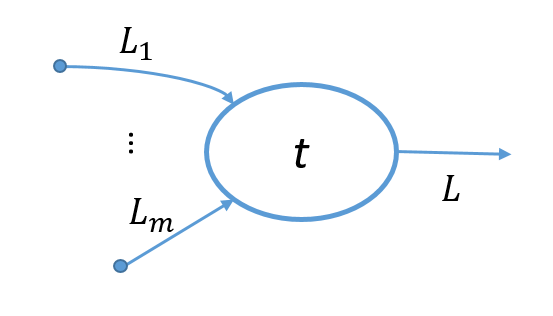
\includegraphics[width=0.3\linewidth]{10-1}
	\caption{технологический процесс}
	\label{fig:10-1}
\end{figure}
$t:L_1\wedge \ldots\wedge L_m\to L$\\
``$\to$'' - это символ тоже самое, что ``$\supset$''.\\
$L_1,\ldots,L_n$ - входные продукты (материалы). $L$ - выходной продукт (что получится, если на входы $t$ подать материалы $L_1,\ldots,L_m$).
\begin{example}
	$t_1:L_1\to L$, $L_1$ - дерево, $L$ - доски. $t_1$ - распилить дерево на доски.\\
	$t_2:\{L,L_2,L_3 \}\to L_4$, $L_2$ - клей, $L_3$ - шурулы, $L_4$ - стол. $t_2$ - из досок с помощью клея и шурулов сделать стол.
\end{example}
Заметим, что Н-формулы могут иметь более сложный вид: 
\begin{equation*}
t:L_1\vee \ldots\vee L_n\to \Phi_1\vee\ldots\vee \Phi_s
\end{equation*}
Мы будем их рассматривать как множество формул.
\begin{equation*}
t^{'},t^{''},\ldots,t^{(n)}\left\{\begin{array}{l}
L_1\vee \ldots\vee L_n\to \Phi_1\\
\ldots\\
L_1\vee \ldots\vee L_n\to \Phi_n
\end{array}\right.
\end{equation*}
Из процессов $t_1,\ldots,t_l$ можно строить более сложные (составные процессы). В примере 10.1: $t_2:\{L_1,L_2,L_4 \}\to L_4\vee L_5$, где $L_5$ - шкаф. Тогда $\{L_1,L_2,L_4 \}\to \text{стол}: t_2,\quad \{L_1,L_2,L_4 \}\to \text{шкаф}: t_2^{'}$.
%%%
%%%fig 10-2
%%%
\begin{figure}[!htp]
	\centering
	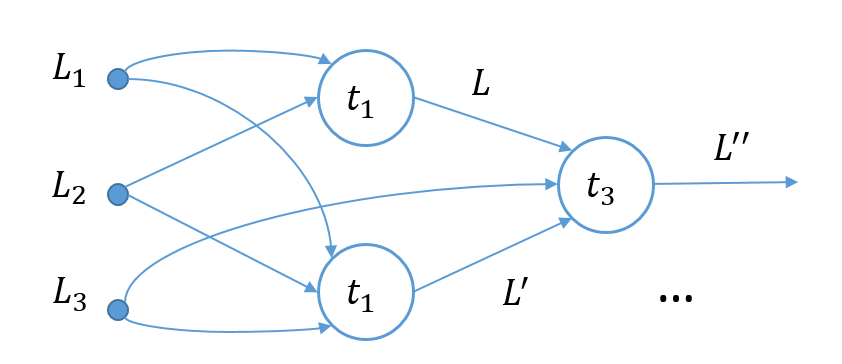
\includegraphics[width=0.3\linewidth]{10-2}
	\caption{сетевой график}
	\label{fig:10-2}
\end{figure}
Если $t_1,\ldots,t_n$ - интерпретировать как время, необходимое для изготовления продукта, то получается сетевой график.\\
Пусть есть БД, которая содержит исходные материалы (продукты). БД=$\{A,B,C,E,H,G\}$ и есть база знаний (содержит информацию о процессах $t_1,\ldots,t_n$). Например, БЗ =$\{t_1:F\wedge B\to E,t_2:C\wedge D\to F,t_3:A\to D \}$.
\begin{question}
	Можно ли получить $Z$, используя БД и БЗ?
\end{question}
\underline{\textbf{Прямой процесс (вывод)}}\\
$t_3:\underbrace{A,A\to D}_{D}\Rightarrow \text{БД}_1=\text{БД}\cup\{ D\}$.\\
$t_2:\underbrace{C,D,C\wedge D\to F}_{F}\Rightarrow \text{БД}_2=\text{БД}_1\cup\{ F\}$.\\
$t_3:\underbrace{F,B,F\wedge B\to Z}_{Z}\Rightarrow Z\text{ можно получить из БД используя процессы } t_3\to t_2\to t_1$.\\

\begin{figure}[!htp]
	\centering
	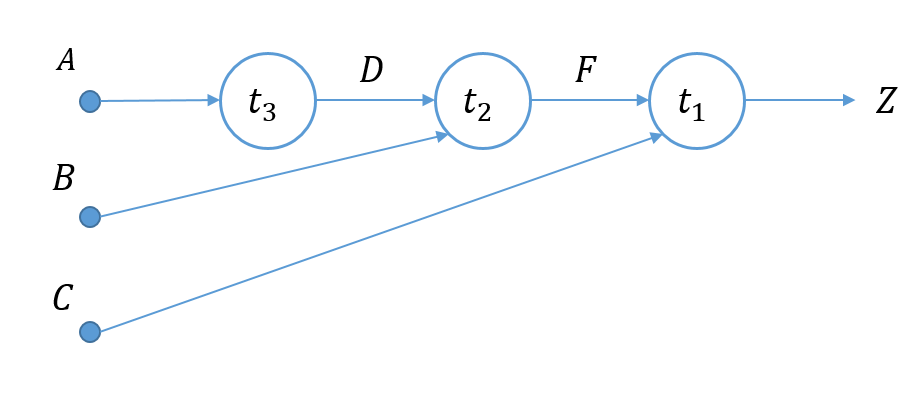
\includegraphics[width=0.3\linewidth]{10-3}
	\caption{прямой процесс}
	\label{fig:10-3}
\end{figure}
$\text{БД}_i$ - состояния БД на $i$-ом шаге.\\
$\text{БД}_i=\text{БД}_{i-1}\cup \{\text{результат применения БЗ к БД}_{i-1};\}$.\\
$\text{БД}_0$ - начальное состояние.\\
\\
\underline{\textbf{Обратный процесс(вывод)}}\\
Ищем в БЗ продукцию, в правой части которой стоит $Z$. Если такой продукции нет, то ответ отрицательный ($Z$ получить нельзя).\\
Есть в БЗ. (см. рис. обратный процесс).\quad 
%%
%%fig
%%
\begin{figure}[!htp]
	\centering
	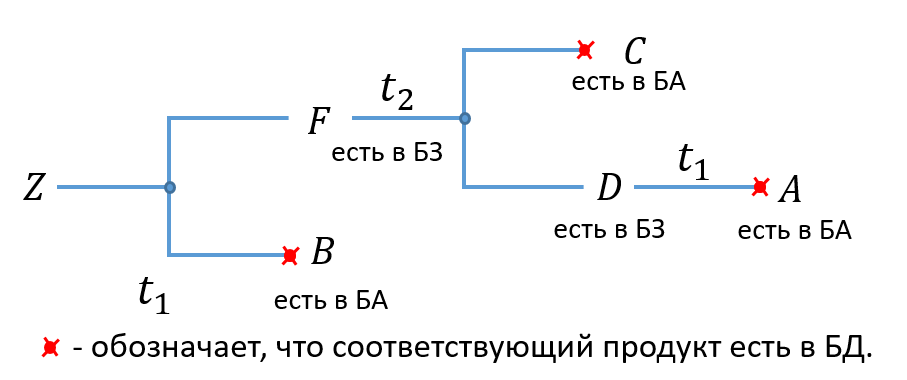
\includegraphics[width=0.5\linewidth]{10-4}
	\caption{обратный процесс}
	\label{fig:10-4}
\end{figure}
* - обозначает, что соответствующий продукт есть в БД. Т.к. все концевые вершины (листья) дерева $T$ помечены ``*'', то $Z$ получить можно.\\
\\
\underline{\textbf{Масштабирование задачи-десятки тысяч материалов и миллионы процессов}}.\\
Рассмотрим более сложный
\begin{example}
	БД = $\{A_1,A_2,A_3.A_4,A_5,A_9 \}$\\
	БЗ = $\{A_1\wedge A_2\wedge A_3\to A_{10};A_3\wedge A_1\to A_7;A_2\wedge A_5\wedge A_1\to A_6; A_9\wedge A_8\wedge A_7\to A;A_1\wedge A_3\to A_9;A_1\wedge A_4\wedge A_6\to A_8\}=\{t_1,t_2,t_3,t_4,t_5,t_6 \}$.\\
	Можно ли получить $A$ из \{БД\} и \{БЗ\}?
\end{example}
 %%
%%
%%
Заметим что $\forall$ $H$-формулу легко преобразовать в дизъюнкт:\\
$(L_1 \land ...\land L_n \to L)=(\overline{L_1\land L_2 \land ... \land L_n})\lor L= \bar{L_1}\lor \bar{L_2}\lor ... \lor \bar{L_n}\lor L$ и далле, преобразовать все наши $H$-формулы в обычные дизъюнкты, можно применять известные нам резолютивиые($Res$) процедуры вывода.\\
Трудности:
\begin{figure}[!htp]
	\centering
	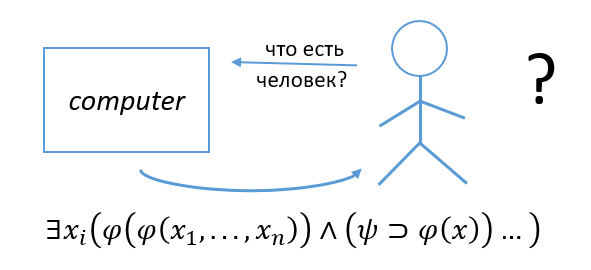
\includegraphics[width=0.4\linewidth]{10-5}
	\caption{трудность}
	\label{fig:10-5}
\end{figure}
Как перевести с языка формул на естественный язык?
\begin{question}
	Истинна ли формула $\text{ЧЕТ}(x)\supset \text{ЧЕТ}(x+1)$\\
	\centerline{где $\text{ЧЕТ}(x)=\left\{
		\begin{array}{l}
		1 \text { если } $x=2k$\\
		0 \text{ если } $x=2k+1$ \text{  }k=0,1,2...
		\end{array}\right.$}
\end{question}
\underline{\textbf{Трехзначные логики}}\\
$\{\underbrace{0}_{\text{ложь}},\underbrace{1}_{\text{неопределено}},\underbrace{2}_{\text{истина}}\}$
\begin{figure}[!htp]
	\centering
	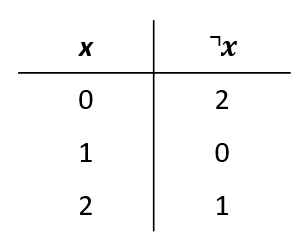
\includegraphics[width=0.2\linewidth]{10-6}
	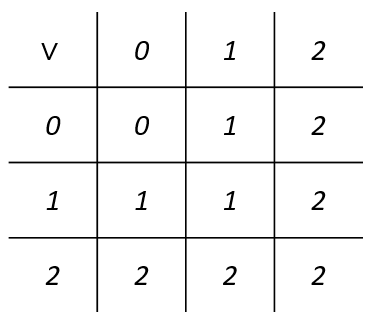
\includegraphics[width=0.2\linewidth]{10-7}
	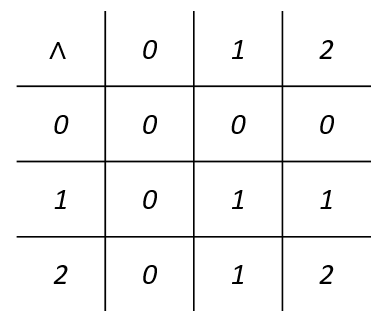
\includegraphics[width=0.2\linewidth]{10-8}
	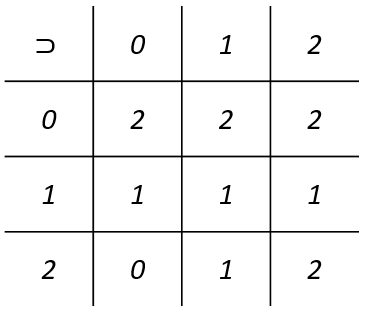
\includegraphics[width=0.2\linewidth]{10-9}
	\caption{трехзначные логики}
\end{figure}
Оказывается что $\supset$ сложно выражается через аналоги $\lnot, \land $ и $\lor$\\
$(x\supset y)=\lnot \lnot(x\lor \lnot \lnot x)\lor (x \land \lnot \lnot x)\lor (\lnot \lnot(\lnot x \lor \lnot \lnot x)\land y)$\\
\begin{Remark} см. рис.
	\begin{figure}[!htp]
		\centering
		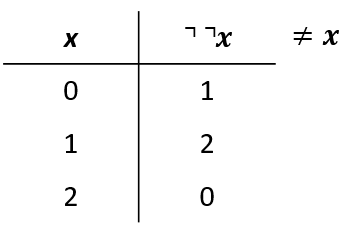
\includegraphics[width=0.3\linewidth]{10-10}
		\caption{замечание 10.1}
		\label{fig:10-10}
	\end{figure}
\end{Remark}
О языке $PROLOG$ - язык, использующися синтаксис и семантику языка исчисления предикатов.\\
Аксиомы языка $PROLOG$-факты.
\begin{example}
	$F(A,B)=A$ отец $B$.\\
	$M(A,B)=A$ мать $B$.\\
	$W(A)=A$ - женщина.\\
	....
\end{example}
База данных: БФ=$\{\text{факт 1},...,\text{факт N}\}$ - база фактов.\\
База значение: БП=$\{\text{правила 1},...,\text{правила K}\}$ - база правил.\\
БФ=$\{\text{A отец Б},\text{Б мать В},\text{В мать Г},\text{Г родитель Д},\text{Г - женщина}\}$\\
БП=$\{\circled{1} x \text{ родитель } y \text{ если } x \text{ отец } y,\circled{2} x \text{ родитель } y \text{ если } x \text{ мать } y,$\\
$\circled{3} x \text{ дедушка } y \text{ если } (x \text{ отец } z)\land (z \text{ родитель } y),\circled{4} x \text{ бабушка } y \text{ если } (x \text{ мать } z)\land (z \text{ родитель } y),$\\
$\circled{5} x \text{ предок } y \text{ если } x \text{ родитель } y,\circled{6} x \text{ предок } y \text{ если } (x \text{ родитель } z)\land (z \text{ предок } y),$\\
$\circled{7} x \text{ мать } y \text{ если } (x \text{ родитель } y)\land (x \text{ женщина}),\circled{8} x \text{ отец } y \text{ если } (x \text{ родитель } y)\land (x \text{ мужчина})\}$\\
\textbf{Запрос:} $A$ родитель $Б$?\\
Интерпретатор $PROLOGF$ обращается к БФ и ищет запрос \underline{с начала}.\\
Среди фактов. Факта ``A радитель Б'' нет. Далее он ищет подходящее правило:\\
если $x:=\text{А}, y:=\text{Б}$ то правино $\circled{1}$ из БП:\\
А родитель Б если (А отец Б). Далее нам надо ``доказать'' чть (А отец Б) но такой факт есть в БФ $\rightarrow$ ответ на запрос ``А родитель Б''- ``ДА''.\\
Более сложно получтиь польжительный ответ на запрос ``А предок Д''? Здесь придется перебирать правила $\circled{1}-\circled{8}$, прежде чем путем подстановок констант A и Д получться отве ``ДА''.
\begin{Remark}
	Попробуите самостоятельно получить ответ на этом запрос.
\end{Remark}
\textbf{Очень Важный факт}\\
Не существуем интерпретатора(алгоритма), который для любой $PROLOG$-программы и любого ДА/НЕТ запрос позволяет за конечное время(число шатов) получить ответ(``ДА'' или ``НЕТ'')\\
Сравни с существованием универсальной машиный Тьюринга!
\section{Лекция 11}
\underline{\textbf{Об экспертных системах}}\\
Рассмотрим слова = \{ мама, папа, дом, ложка, вилка, кино, домино, печь, ночь, киль, шпиль, лекарь, токарь\}. Это слово в именительном падаже. (отвечают на вопрос ``кто?'' ``что?''). Надо написать алгоритм, преобразующий слова в родительный падеж (отвесает на вопросы ``кого нет?'' ``чего нет?''). В таком преобразований меняются \underline{только окночание} слова. Как меняются окночания этих слов в родительном падеже?\\
\{мамы, папы, дома, ложки, вилки, кино, домино, печи, ночи, киля, шпиля, лекаря, токаря \}.\\
Видим, что ``кино'' и ``домино'' не меняются. (см. Блок-схема)\\
мама, папа: А$\to$Ы,\quad лекарь, токарь: АРЬ$\to$АРЯ, \quad ложка, вилка: КА$\to$КИ.\\
ночь, печь: ЧЬ$\to$ЧИ,\quad шпиль, киль: Ь$\to$Я.\\
\\
\begin{figure}[!htp]
	\centering
	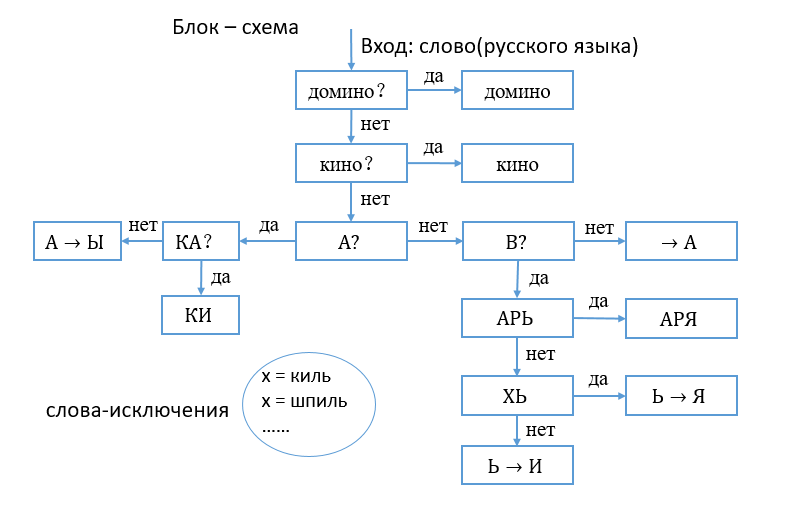
\includegraphics[width=0.6\linewidth]{11-1}
	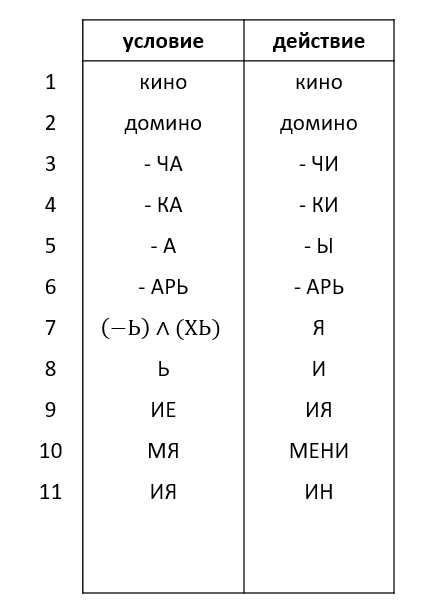
\includegraphics[width=0.3\linewidth]{11-2}
	\caption{Блок-схема и продукционные системы}
	\label{fig:11-1}
\end{figure}
Как изменить алгоритм (блок-схему), если добавляются слова\\ \{отношение, время, реакция, индукция, задача, функция\} - именительный падеж.\\
\{отношения, времени, реакции, индукции, задачи, функции \}.\\
Алгоритм изменить несложно, но придётся переделывать(перепрограммировать) алгоритм. \\
Другая идея - использовать продукционные системы Если <условие> то <действие>. (см. \ref{fig:11-1} справа)\\
* - слова-исключения=\{киль,шпиль\}.\\
Легко добавлять новые продукции. Механизм вывода не меняется.\\
\underline{Статика} - алгоритм. \underline{Динамика} - алгоритм на основе продукций.\\
\\
\underline{\textbf{Масштабирование задачи}}\\
(миллионы банковских транзакций в день). Язык продукций лежит в основе многих экспертных систем.\\
\underline{\textbf{Задача дискретной оптимизации}}
\begin{enumerate}
	\item Задача оптимизации - это последовательность $PR$ =\{$T_1,T_2,\ldots$\} индивидуальных (конкретных) задач, получающихся из $РR$ при конкретном выборе числовых параметров, участвующих в постановке задачи. $T_i\in$PR, $T_i$ - индивидуальная задача.
	\item $\forall T_i$ определена совокупность (множество) $R$ допустимых решений $r$ этой задачи.
	\item Каждое решение $r\in R$ характеризуется сложностью $l(r)$ - как правило целое число.
\end{enumerate}
В задаче оптимизации требуется по произвольной $T_i\in PR$ найти алгоритм, который бы находил решение $r$ с оптимальным ($l(r)\to \min$ - задача на поиск минимума, или $l(r)\to \max$ - задача на поиск максимума) значением $l(r)$.

Будем рассматривать эти задачи в форме вопроса ``верно ли, что для данной индивидуальной задачи $T_i\in PR$ и заданного значения $l$ существует такое решение $r_i\in R$, что $l(r_i)\leqslant l$(или $l(r)\leqslant l$ в задаче на максимум)''. Ответом на вопрос будет ``да'' или ``нет''.

\underline{\textbf{Кодирование задачи}}\\
Входами в задачах дискретной оптимизации могут быть графы, матрицы, булевы функции, дизъюнкты и.т.д. Предпологаем, что они как-то закодированы в виде наборов нулей и единиц (например так, как их кодируют в компьютере). Такой код имеет определенную длину $n$ (например, число бит или байт), необходимо для представления задачи в компьютере. Кодирование может быть разным (коды одной задачи могут иметь разную длину $n_1,n_2,\ldots$), но как правило для $n_1,n_2$ можно указать такие полиномы $P_1$ и $P_2$, что $n_1\leqslant P_1(n_2)$, и $n_2\leqslant P_2(n_1)$. То есть ``перекодирование'' одного кода в другой требует не больше, чем полином шагов.
\begin{definition}
	\textbf{Класс P} - класс дискретных задач (в форме распознавания), для которых существуют алгоритмы, решающие эти задачи за число шагов $\leqslant$ некоторый полином от размера входа задачи.
\end{definition}
\begin{figure}[!htp]
	\centering
	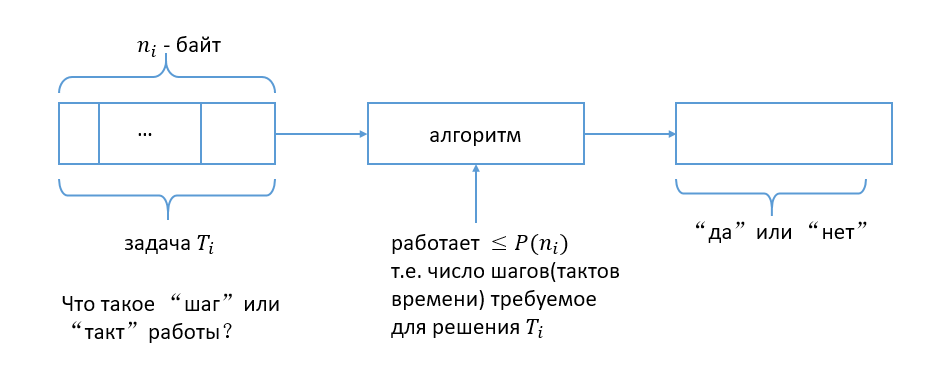
\includegraphics[width=0.8\linewidth]{11-3}
	\caption{Кодирование задачи}
	\label{fig:11-3}
\end{figure}
Что такое ``шаг'' или ``такт'' работы?. Класс $PR\ne \emptyset$, этому классу принадлежит задача о построении минимального остовного дерева графа $G$.
\begin{definition}
	\textbf{Класс NP} - это задачи, для которых
	\begin{enumerate}
		\item Существует алгоритм (переборного типа), решающий эту задачу.
		\item Мы не знаем, есть ли алгоритм, решающий эту задачу ``лучше'' (например за полином шагов от размера входа)
		\item Если нам предъявлены набор значений(возможное решение задачи), то мы за полином шагов можем сказать, является ли это решением задачи (``да'' или ``нет'')
	\end{enumerate}
\end{definition}
Позже мы покажем, что класс $NP$ тоже не пуст.
\begin{figure}[!htp]
	\centering
	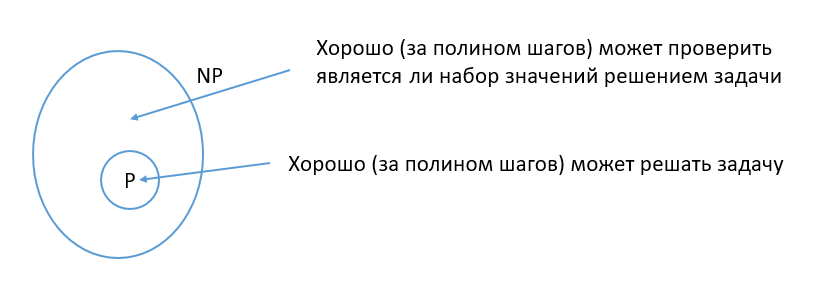
\includegraphics[width=0.7\linewidth]{11-4}
	\caption{$P$ и $NP$}
	\label{fig:11-4}
\end{figure}

\textbf{ГЛАВНЫЙ ВОПРОС:} $P?=NP$.\\
\\
\underline{\textbf{Задача о покрытии таблицы:}}
\begin{figure}[!htp]
	\centering
	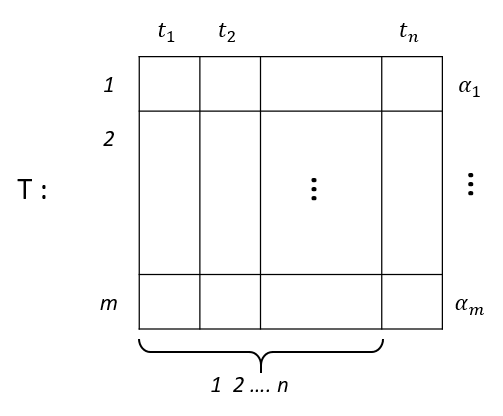
\includegraphics[width=0.4\linewidth]{11-5}
	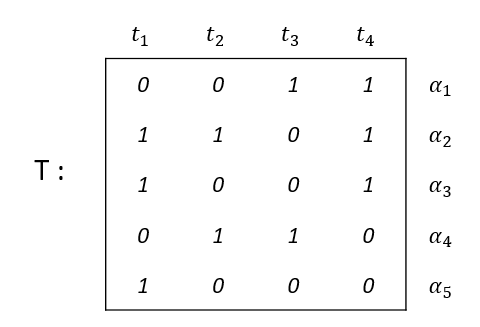
\includegraphics[width=0.4\linewidth]{11-6}
	\caption{Задача о покрытии таблицы и пример \ref{example-11-1}\ref{example-11-2}}
	\label{fig:11-5}
\end{figure}

Таблица из $0,1$ размера $m\times n$ без строк целиком нулевых.
\begin{definition}
	Говорим, что стоблец \textbf{покрывает} строку, если на их пересечении в таблице $T$ стоит единица.
\end{definition} 
\underline{Задача.} Найти покрытие всех строк таблицы $T$ столбцами $t_{i_1},\ldots,t_{s}\subseteq\{t_1,\ldots,t_n\}$ так, чтобы $s$ было минимальным.
\begin{example}(СМ. рис. \ref{fig:11-5} справа)\\
	\label{example-11-1}
	$t_1,t_3$ образуют оптимальное покрытие строк таблицы $T$ ($m\cdot n$) - размер входа задачи $T$.
\end{example}
Эта задача $\in NP$:
\begin{enumerate}
	\item Есть переборный алгоритм = $2^n$ шагов.
	\item Неизвестен алгоритм лучше чем перебор (в частности неизвестно, есть ли полиноминальый алгоритм)
	\item Если дан набор столбцов $t_{i_1},\ldots,t_{i_p}$, то проверить, является ли он покрытием $T$ (покрывает ли он все строки) можно сделать за $O(\underbrace{m\cdot p}_{\text{размер входа}})$ шагов. Шаг - это одно сравнение между собой элементы строки и столбца.
\end{enumerate}
\underline{\textbf{Эвристический (приближенный) алгоритм решения задачи о покрытии таблицы.}}
\begin{definition}
	Число единиц в столбце $l_i$ называется его \textbf{весом} и обозначается $w_i=w(l_i)$.
\end{definition}
АЛГОРИТМ:
\begin{enumerate}
	\item В таблице $T$ берем столбец $l_i$ наибольшего веса. Если их несколько, то берем любой из них.
	\item Вычеркиваем из $T$ все строки, накрытые $l_i$ и сам столбец $l_i$, получим таблицу $T_1$
	\item Далее с таблицей $T_1$ проделываем шаги $1$ и $2$. Получим $T_2$.
	\item $\ldots\ldots$
\end{enumerate}
Условие останова: в очередной подтаблице $T^{'}$ все строки вычеркнуты.
\begin{example}(СМ. рис. \ref{fig:11-5} справа)
\label{example-11-2}
$t_1$ и $t_2$ - столбцы наибольшего веса $w(t_1)=w(t_n)=3$. Берем $t_1$ и вычеркиваем строки $\alpha_2,\alpha_3,\alpha_5$ и сам столбец. После вычеркивания $\alpha_1,\alpha_4$ и $t_3$. Больше строк нет. Итак, $t_1,t_3$ \underline{оптимальное покрытие}.
\begin{displaymath}
\mathbf{T_1} :
 \begin{array}{cccc}
 & t_{2} & t_{3} &t_4 \\
\alpha_{1} & 0 & 1& 1 \\
\alpha_4 & 1 & 1& 0
\end{array} ,\quad w(t_3)=2.
\end{displaymath}
\end{example}
Посмотрим (опять рис. \ref{fig:11-5} справа), что произойдет, если в качестве начального взять столбец $t_4 (w(t_4)=3)$. Вычеркиваем $t_4$ и строки $\alpha_1,\alpha_2,\alpha_3$, накрытые им, получим $T_1$. После этого заметим, что все столбцы веса $1$. Берем $t_3$ - вычеркиваем его и строку $\alpha_4$, получим $T_2$. Здесь берем $t_1$(он накрывает $\alpha_5$). Все строки накрыты. $\Rightarrow$ Ответ: $t_4,t_3,t_1$. - не оптимальное.
\begin{displaymath}
\mathbf{T_1} :
\begin{array}{cccc}
& t_{1} & t_{2} &t_3 \\
\alpha_{4} & 0 & 1& 1 \\
\alpha_5 & 1 & 0& 0
\end{array} ,\quad 
\mathbf{T_2} :
\begin{array}{ccc}
& t_{1} & t_{2}  \\
\alpha_{5} & 1 & 0
\end{array}
\end{displaymath}
Проверить, является ли $\{t_2,t_3,t_4\}$ покрытием $T$ (самостоятельно).

Рассмотрим теперь таблицу (рис. \ref{fig:11-7})следующего вида: она состоит из трех подтаблицы\\
\begin{figure}[!htp]
	\centering
	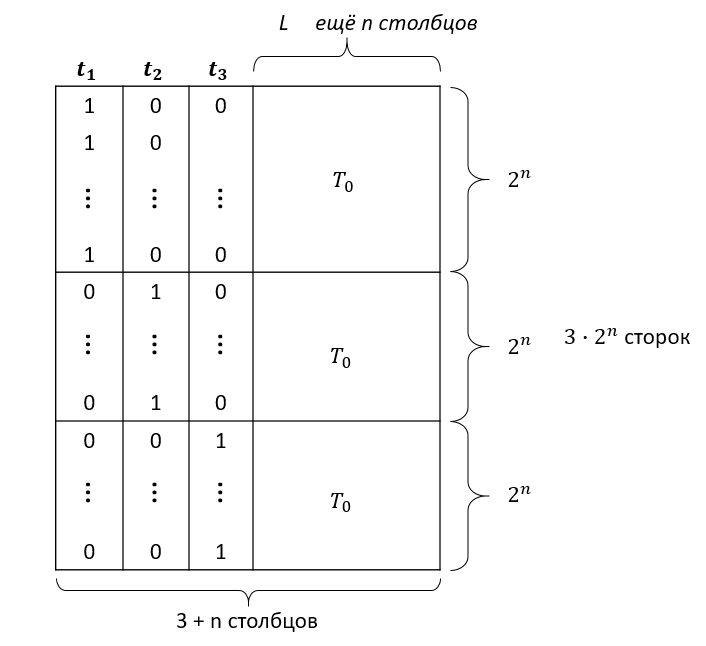
\includegraphics[width=0.5\linewidth]{11-7}
	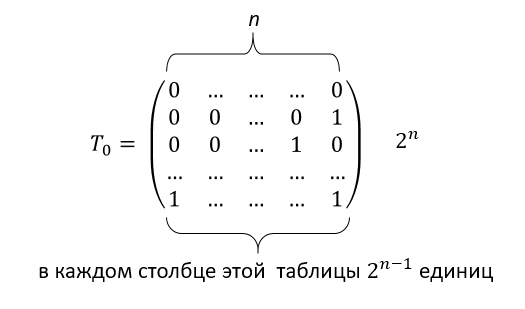
\includegraphics[width=0.45\linewidth]{11-8}
	\caption{Таблица специального вида}
	\label{fig:11-7}
\end{figure}
В первом столбце $2^n$, во втором столбце $2^n$, в третьем столбце $2^n$. -----> единиц\\
В четвертом  $3\cdot 2^{n-1}$, в пятом $3\cdot 2^{n-1}$.\\
\ldots\\
В $n+4$ : $3\cdot 2^{n-1}$ единиц.\\
Эвристический алгоритм выберет в качестве покрытия столбцы с номером $4,5\ldots,n+4$, т.к. их вас будет $3\cdot 2^{n-1}>2^n$ - вес первого, второго и третьего столбца.
\begin{Remark}
	Легко видно, что столбец $1,2,3$ является оптимальным решением задачи о покрытии.
\end{Remark}
Такие алгоритмы называются \textbf{жадными} (greedy).

\section{Лекция 12}
\underline{\textbf{Содержательно:}} проблема $PR_1$ сводится к проблеме $PR_2$, если алгоритм решения проблемы $PR_2$ может быть использован и для решения $PR_1$.\\
\underline{\textbf{Формально:}} 
\begin{definition}
	Пусть $PR_1$ и $PR_2$ - две дискретные задачи в форме распознавания (т.е. ответом в них будет ``да'' или ``нет''). Задача $PR_1$ \textbf{полиномиально} сводится к задаче $PR_2$, если для некоторого полинома $P_i$ по любой индивидуальной (конкретной) $T_i^{'}\in PR_1$ можно построить за $P(|T_i^{'}|)$ число шагов индивидуальную задачу $T_i^{''}\in PR_2$ так, чтобы ответы в задачах $T_i^{'}$ и $T_i^{''}$ совпадали (или оба ответа ``да'' или оба ответа ``нет'').
\end{definition}
\underline{Обозначение} $PR_1\mapsto PR_2$. $|T_i^{'}|$ - размер \underline{входа} задачи $T_i^{'}$.

Заметим, что отношение ``$\mapsto$'' транзитивно
\begin{equation*}
T_i\underbrace{\mapsto}_{P_1(|T_i|)\text{ полином 1}} T_i^{'}\underbrace{\mapsto}_{P_1(|T_i^{'}|)\text{ полином 2}} T_i^{''} \quad \Rightarrow\quad  T_i\mapsto T_i^{''}.
\end{equation*}
Заметим, что \underline{подстановка} полинома $P_2(P_1(T_i))$ в полином будет опять полиномом. Отсюда следует, что если $PR_1\mapsto PR_2$ и $PR_2\in$ классу $P$, то и $PR_1$ тоже $\in P$ (класс задач, решаемых за полиномиальное (от размера входа) число шагов).

На предыдущей лекции мы рассматривали задачу о покрытии таблицы набором столбцов. А в начале курса мы исследовали задачу о выполнимости набора дизъюнктов $D_1,\ldots,D_n$. (Нас интересовало выполнима формула $D_1,\ldots,D_n$ или нет). Нетрудно убедиться, что обе задачи принадлежат классу $NP$.
\begin{enumerate}
	\item Их можно решить перебором всех подмножеств столбцов - $2^m$ вариантов (или перебором всех значений переменных, входящих в формулу $K(x_1,\ldots,x_s)=D_1\wedge\ldots\wedge D_p$ - $2^s$ вариантов).
	\item Нам не известен алгоритм решения этой задачи, лучший, чем перебор вариантов (например, полиномиального типа).
	\item Если нам задан набор столбцов $l_1,\ldots,l_p$, $p\leqslant m$ (набор значений переменных $x_1=\alpha_1,\ldots,x_n=\alpha_n(\alpha_i\in\{0,1\})$), то ответ на вопрос задач занимает не более чем $O(|T|)$ шагов, где $T$ или задача о покрытии или задача о выполнимости КНФ $K(x_1,\ldots,x_n)=D_1\wedge\ldots\wedge D_p$.
\end{enumerate}
\begin{theorem}
	Задача о выполнимости полиномиально сводится к задаче о покрытии талблиц.\\
	Коротко: Задача о выполнимости $\mapsto$ задаче о покрытии.
\end{theorem}
\emph{Доказательство.} Пусть $K(x_1,\ldots,x_n)=D_1\wedge\ldots\wedge D_m$ - КНФ. Построим таблицу $T_k$, которая имеет $2n$ столбцов, обозначенных $x_1,\ldots,x_n,\bar{x}_1,\ldots,\bar{x}_n$, и $n+m$ строк.
\begin{figure}[!htp]
	\centering
	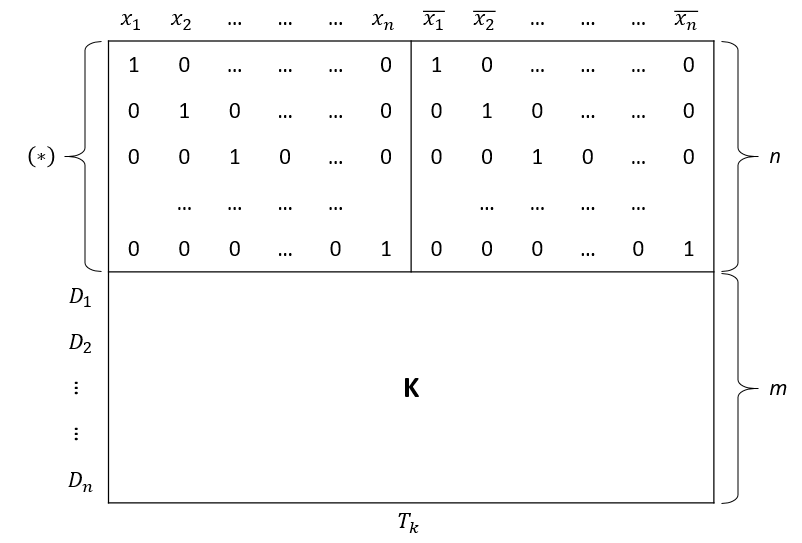
\includegraphics[width=0.7\linewidth]{12-1}
	\caption{Таблица $T_k$}
	\label{fig:12-1}
\end{figure}
 Строки (*) называются вспомогательными. Правило заполнения $T_k$ в области $K$: Если переменная $x_i^{\delta}$ входит в дизъюнкт $D_j$, то на пересечении столбца $x_i^{\delta}$ и $j$-ой строки ставится $1$, в противном случае $0$; $j=1,\ldots,m,\delta\in\{0,1\},i=1,\ldots,n$.
 \begin{example}
 	\begin{figure}[!htp]
 		\centering
 		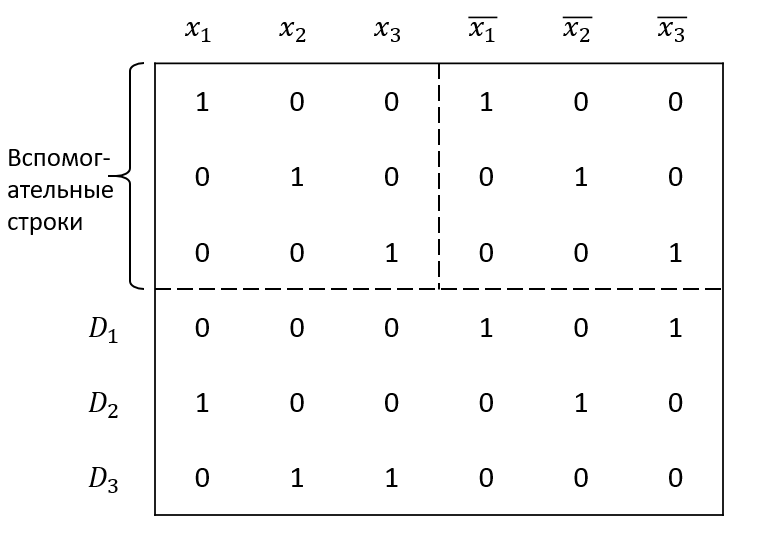
\includegraphics[width=0.5\linewidth]{12-2}
 		\caption{Таблица к примеру}
 	\end{figure}
 	\label{ex-12-1}
 	$K=(\underbrace{\bar{x}_1\vee \bar{x}_3}_{D_1})\wedge (\underbrace{x_1\vee \bar{x}_2}_{D_2})\wedge(\underbrace{x_2\vee x_3}_{D_3})$.
 \end{example}
ВАЖНО: Если какие-то $n$-столбцов образуют покрытие всех вспомогательных строк, то каждая $i$ вспомогательная строка накрыта или $x_i$ или $\bar{x}_i$ - в противном случае, (т.к. в покрытии $n$ столбцов) какая-то переменная не будет участвовать в покрытии и соответствующая строка не будет накрыта.

Следовательно, любое покрытие $T_k$, состоящее из $n$ столбцов (если оно существует) имеет вид $\{x_1^{\alpha_1},\ldots,x_n^{\alpha_n} \}$ - все переменные разные.
\begin{Remark}
	Дальше будем считать, что нужное покрытие состоит ровно из $n$ столбцов, т.к. если есть покрытие из $l<n$ столбцов, то добавляя к $l$ столбцам ещё какие-то $n-l$ столбцов мы получим тоже покрытие.
\end{Remark}
Каждое покрытие строк $T_k$ столбцами имеет вид $\{x_1^{\alpha_1},\ldots,x_n^{\alpha_n} \}$. Каждая строка $D_i$ ``пересекается'' по единице с некоторым столбцом $x_i^{\alpha_i}$. Тогда при $x_i^{\alpha_i}=1$ (т.е. $x_i=\alpha_i$) получим, что $D_j=1$.

Полагая $x_1=\alpha_1,x_2=\alpha_2,\ldots,x_n=\alpha_n$ получим что $D_1=1,D_2=1,\ldots,D_m=1\Rightarrow K(x_1,\ldots,x_n)=D_1\wedge\ldots\wedge D_m=1$, т.е. КНФ выполнима, т.е. если $\{x_1^{\delta_1},\ldots,x_n^{\delta_n} \}$ покрытие $T_k$, то $K(x_1,\ldots,x_n)$ выполнима.

\underline{Обратно:} Пусть $x_1=\alpha_1,\ldots,x_n=\alpha_n$ и на нем $K(\alpha_1,\ldots,\alpha_n)=1$. Тогда $\{x_1^{\alpha_1},\ldots,x_n^{\alpha_n} \}$ образует покрытие $T_k$. 

В самом деле: $K(\alpha_1,\ldots,\alpha_n)=1\Rightarrow D_1=1,\ldots,D_n=1$, т.е. в каждой строке, соответствующей $D_1,\ldots,D_n$ есть хотя бы одна единица и $i$-ую вспомогательную строку, т.е. если КНФ$(\alpha_1,\ldots,\alpha_n)$ выполнима, то $\{x_1^{\alpha_1},\ldots,x_n^{\alpha_n} \}$ покрытие таблицы. 

Теорема доказана. $\qedsymbol$

Вернемся к нашему примеру \ref{ex-12-1}.
\begin{enumerate}
	\item $\{\bar{x}_1,\bar{x}_2,x_3 \}$ образуют покрытие всех строк таблицы. $\{x_1=0,x_2=0,x_3=1 \}$ обращают $K(x_1,x_2,x_3)=1$: $K(0,0,1)=(\bar{0}\vee \bar{1})\wedge(0\vee \bar{0})\wedge(0\vee 1)=1$.
	\item Возьмем набор значений переменных: $x_1=1,x_2=1,x_3=0\Rightarrow K(1,1,0)=1$. Тогда $\{x_1,x_2,\bar{x}_3 \}$ - эти столбцы накрывают все строки таблицы.
\end{enumerate}
Итак, зная ответ на вопрос ``существует ли покрытие таблицы из $n$ столбцов'', мы можем ответить и на вопрос ``выполнима ли КНФ $K(x_1,\ldots,x_n)$'' и наоборот.

Идея сводимости за полином шагов приводит к следующей проблеме: Существуют ли проблемы $PR$, к которым полиномиально сводятся все остальные $PR_i$ ($PR$ и $PR_i$ конечно $\in NP$).
\begin{definition}
	\begin{figure}[!htp]
		\centering
		\includegraphics[width=0.5\linewidth]{12-3}
		\caption{Класс $NP$}
	\end{figure}
	$\forall PR\in NP\quad (PR_i\mapsto PR\in NP)$. Такая задача $PR$ (если она существует) будет называется \textbf{NP-полной} задачей.
\end{definition}
Исторически оказалось, что первой $NP$-полной задачей оказалось задача о выполнимости КНФ $K=D_1\wedge\ldots\wedge D_n$. Подумайте о связи с резолютивными методами для ИВ. 

Заметим, что вопрос $P=NP$ можно теперь сформулировать так: $P?=NP\Leftrightarrow (\exists PR\in NP\setminus P),PR - NP-\text{полная задача}$.

\underline{\textbf{Алгоритм приближенного решения некоторых $NP$-полных задач.}}\\
\textbf{Задача об упаковки (в контейнеры)}\\
Задано множество $S=\{p_1,\ldots,p_n \}$ - предметы, $\forall p_i$ обладает ``размером'' (``весом'',\ldots) $r_i=r(p_i)$. Если $S^{'}\subseteq S$, то размер (вес) подмножества $S^{'}$ равен сумме размеров (весов), входящих в него предметов (Обозначение: $r(S^{'})$). Требуется найти такое разбиение $S$, что
\begin{enumerate}
	\item $S=S^{1}\cup S^{2}\cup\ldots\cup S^{t},S^{i}\cap S^{j}=\emptyset,i\ne j,i,j=1,\ldots,n.$
	\item $r(S^1)\leqslant 1,\ldots,r(S^t)\leqslant 1$
	\item $t\to \min$
\end{enumerate}
\begin{figure}[!htp]
	\centering
	\includegraphics[width=0.4\linewidth]{12-4}
	\caption{Задача об упаковки}
\end{figure}
Если бы были 1) и 2), то это тривиальное решение. (см. рис.) В задаче предпологается, что $\forall i=1,\ldots,n,r_i=r(p_i)\leqslant 1$. При учете 3) задача становится трудной $(\in NP)$. 

Обозначим через $t_{opt}$ - минимальное число контейнеров единичного размера, в которые можно упаковать(уложить, поместить) все предметы из $S$.
\begin{figure}[!htp]
	\centering
	\includegraphics[width=0.9\linewidth]{12-5}
	\caption{Алгоритм $A_1$}
\end{figure}
Отметим, что при такой укладке только один контейнер может быть заполнен меньше, чем на $1/2$. Т.е. вот такой случай не возможен:
\begin{figure}[!htp]
	\centering
	\includegraphics[width=0.7\linewidth]{12-6}
	\caption{Невозможный случай}
\end{figure}
Наш алгоритм предметы из $j$-го контейнера переместил бы в $i$-й.

Итак, все контейнеры заполнены $>1/2$ и только один будет (возможно) заполнен меньше, чем на $1/2$. Пусть число контейнеров (при укладке этим алгоритмом) будет $l_{A_1}$.
\begin{figure}[!htp]
	\centering
	\includegraphics[width=0.4\linewidth]{12-7}
	\caption{Отбросить последний контейнер}
\end{figure}
Отбросим последний контейнер.
\begin{equation*}
\frac{1}{2}(t_{A_1}-1)\leqslant\sum_{i=1}^{n} r_i=r(p_i)\leqslant l_{\text{opt}}\Rightarrow \frac{1}{2} (t_{A_1}-1)<l_{\text{opt}}\quad \bm{t_{A_1}\leqslant 2 l_{\text{opt}}}
\end{equation*}
Можно доказать, что $l_{A_1}\leqslant \frac{17}{10}l_{\text{opt}}+2$ и $\frac{17}{10}$ неулучшаема!

То есть, в худшем случае алгоритм $A_1$ потребует в $2$ раза больше контейнеров, чем $l_{opt}$.

АЛГОРИТМ $A_2$:
\begin{enumerate}
	\item Отсортируем предметы в порядке убывания их весов $r_{i_1}\geqslant\ldots\geqslant r_{i_n}$
	\item К отсортированной последовательности применим алгоритм $A_1$, т.е. сначала берем самый большой предмет $p_{i_1}$, помещаем его в контейнер, затем берем предмет $p_{i_2}$ и пытаемся поместить его в этот же контейнер. Если не помещается - берем новый контейнер, и.т.д.   
\end{enumerate}
Можно доказать, что
\begin{equation*}
l_{A_2}\leqslant \frac{3}{2} l_{\text{opt}}\text{ и } l_{A_2}\leqslant \frac{11}{9} l_{\text{opt}}+4
\end{equation*}
и константа $\frac{11}{9}$ не улучшаема!
ПРОСЬБА ПОСМОТРЕТЬ САЙТ \url{packer3d.com}!

\section{Лекция 13}
Рассмотрим граф $K_n$, каждому ребру которого приписано число больше нуля, называемое \textbf{весом} ребра, расстоянием между вершинами графа и.т.д. ($K_n=(V,E),|V|=n,E=\{(v_i,v_j) \}$ и $i\ne j$ : нет петель в $K_n$) Предполагается при этом, что выполнено неравенство треугольника, т.е. $\forall$ трех вершин $v_i,v_j,v_k$ графа $K_n$ выполнено
\begin{equation*}
w((v_i,v_k))+w((v_k,v_j))\leqslant w((v_i,v_j))
\end{equation*}
Из нерваенства треугольника следует \underline{обобщенное} неравенство треугольника: $\forall$ вершин $v_i,v_{i_1},\ldots,v_{i_n},v_j$ графа $K_n$ верно
\begin{equation*}
w((v_i,v_j))\leqslant w((v_{i},v_{i_1}))+w((v_{i_1},v_{i_2}))+\ldots+w((v_{i_n},v_{j}))
\end{equation*}
Пусть $T$ - минимальное остовное дерево графа $K_n$ и величина $w(T)=\sum\limits_{\text{по всем }(v_i,v_j)\in T} w((v_i,v_j))$ - минимальна и пусть $\pi$-гамильтонов цикл в $K_n$ наименьшего веса, т.е.
\begin{equation*}
w(\pi)=w((v_{i_1},v_{i_2}))+\ldots+w((v_{i_{n-1}},v_{i_n}))+w((v_{i_n},v_{i_1}))=w_{\text{opt}}
\end{equation*}
Заметим, что $w(T)<w(\pi)$. (т.к. если из цикла удалить одно ребро, то получим остовное дерево, не обязательно минимальное) В остовном дереве $T$ удвоим ребра (сохраняя отметки на ребрах). Теперь степень каждой вершины четна и граф (полученный из $T$ удвоением ребер) связен, а это необходимое домтаточное условие существования в нем эйлерова цикла. Очевидно $w(C)=2w(T)$. Эйлеров цикл проходит каждое ребро графа один раз $\Rightarrow$ значит он проходит и все вершины графа (необязательно один раз). Отметим, в эйлеровом цикле все первые вхождения вершин из $V$.
\begin{equation*}
C=(v_{j_1},\ldots, v_{j_2},\ldots v_{j_n},\ldots)
\end{equation*}
и рассмотрим обход по циклу $\mu=\{v_{j_1},v_{j_2},\ldots,v_{j_n},v_{j_1} \}$. Из обобщенного неравенства треугольника получаем, что $w(\mu)=w((v_{j_1},v_{j_2}))+w((v_{j_2},v_{j_3}))+\ldots+w((v_{j_{n-1}},v_{j_n}))+w((v_{j_n},v_{j_1}))\leqslant w(C)$. Но $w(C)=2w(T)<2w_{\text{opt}}\Rightarrow w(\mu)< 2w_{\text{opt}}$. Заметим, что ``жадный'' алгоритм $g$ ближайшего соседа может сильно ошибаться
\begin{equation*}
w_g \leqslant\frac{1}{2}\left([\log_2 n]+1 \right) w_{\text{opt}}
\end{equation*}
АЛГОРИТМ $g$: (ближайший сосед) находясь в вершине $v_j$ графа $K_n$ перейти в ближайщую (в смысле величины $w((v_j,v_i))$) вершину $v_i$, которую ещё не проходил. 

Можно показать, что существует такой алгоритм посторения гамильтонова цикла $\mu_1$ в $K_n$, что 
\begin{equation*}
w(\mu_1)\leqslant \frac{3}{2} w_{\text{opt}}
\end{equation*} 

\end{document}
